% Appendix 1

\chapter{Results from Python computation} % Main appendix title

\label{Appendix1} % For referencing this appendix elsewhere, use \ref{AppendixA}

%%%%%%%%%%%%%%%%%%%%%%%%%%%%%%%%%%%%%%%%%%%%%%%%%
%Section 1
%%%%%%%%%%%%%%%%%%%%%%%%%%%%%%%%%%%%%%%%%%%%%%%%%
\section{Results in room conditions}

\subsection{Crack length}

\begin{figure}[H]
	\centering
\begin{subfigure}{0.48\linewidth}
	\centering
	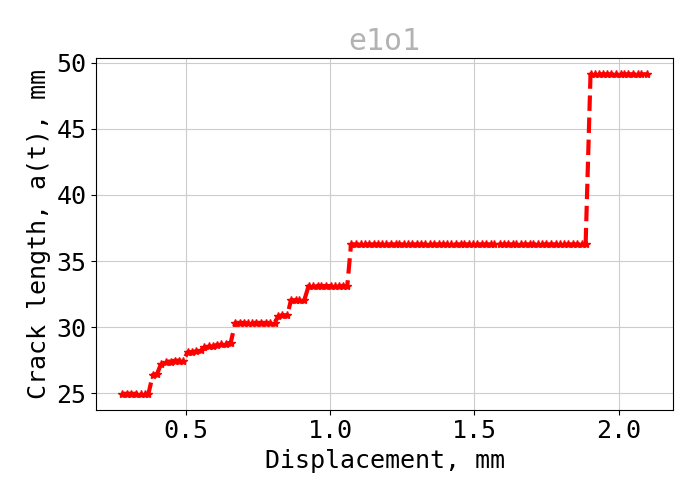
\includegraphics[width=\textwidth]{Figures/e1o1_a}
	\decoRule
	\caption[Crack length E1O1]{Crack length depending on the press displacements, for E1O1 specimen.}
	\label{fig:E1O1_a}
\end{subfigure}
\hfill \\
\begin{subfigure}{0.48\linewidth}
	\centering
	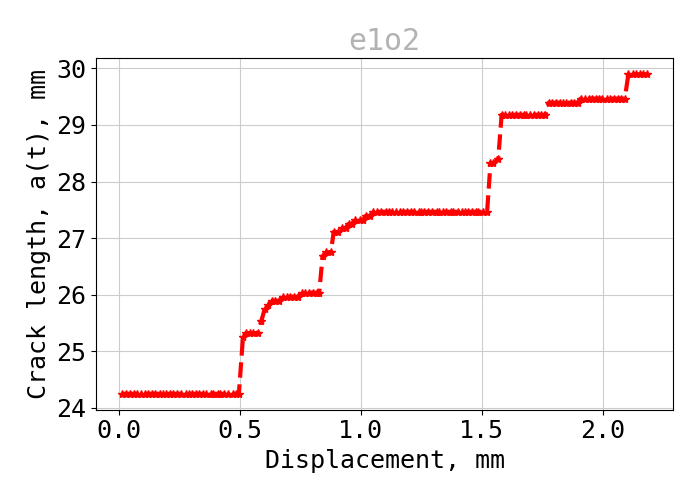
\includegraphics[width=\textwidth]{Figures/e1o2_a}
	\decoRule
	\caption[Crack length E1O2]{Crack length depending on the press displacements, for E1O2 specimen.}
	\label{fig:E1O2_a}
\end{subfigure}
\hfill\\
\begin{subfigure}{0.48\linewidth}
	\centering
	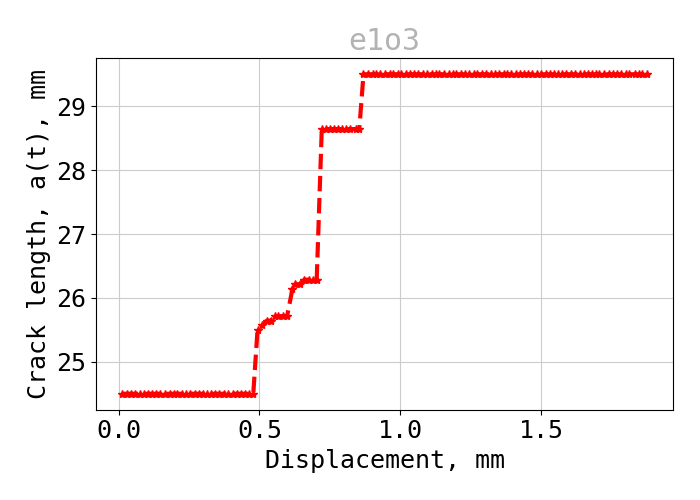
\includegraphics[width=\textwidth]{Figures/e1o3_a}
	\decoRule
	\caption[Crack length E1O3]{Crack length depending on the press displacements, for E1O3 specimen.}
	\label{fig:E1O3_a}
\end{subfigure}
\caption{Crack length evolution on Okoume specimens submitted at room climatical conditions and at an average of 7\% moisture content}
\label{E1o_a}
\end{figure}

\begin{figure}[H]
	\centering
	\begin{subfigure}{0.48\linewidth}
		\centering
		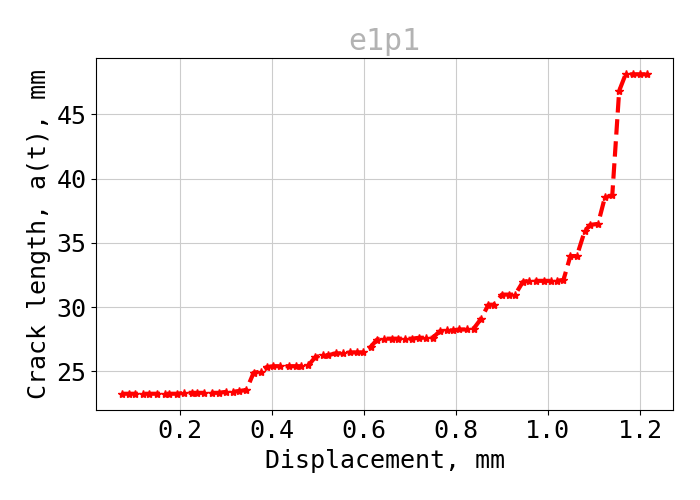
\includegraphics[width=\textwidth]{Figures/e1p1_a}
		\decoRule
		\caption[Crack length E1P1]{Crack length depending on the press displacements, for E1P1 specimen.}
		\label{fig:E1P1_a}
	\end{subfigure}
	\hfill \\
	\begin{subfigure}{0.48\linewidth}
		\centering
		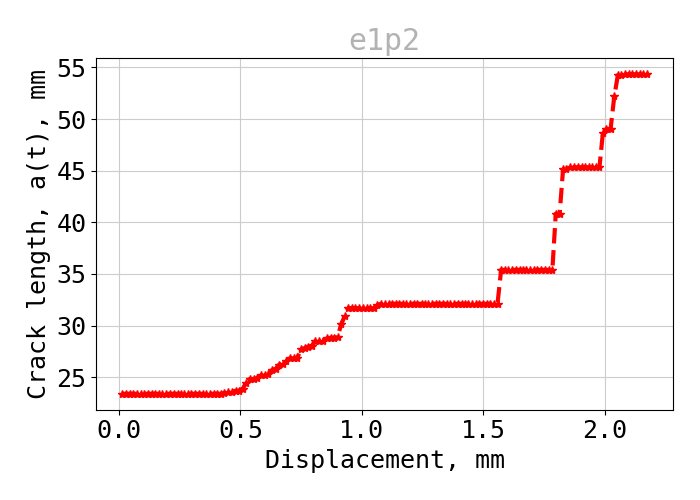
\includegraphics[width=\textwidth]{Figures/e1p2_a}
		\decoRule
		\caption[Crack length E1P2]{Crack length depending on the press displacements, for E1P2 specimen.}
		\label{fig:E1P2_a}
	\end{subfigure}
	\hfill\\
	\begin{subfigure}{0.48\linewidth}
		\centering
		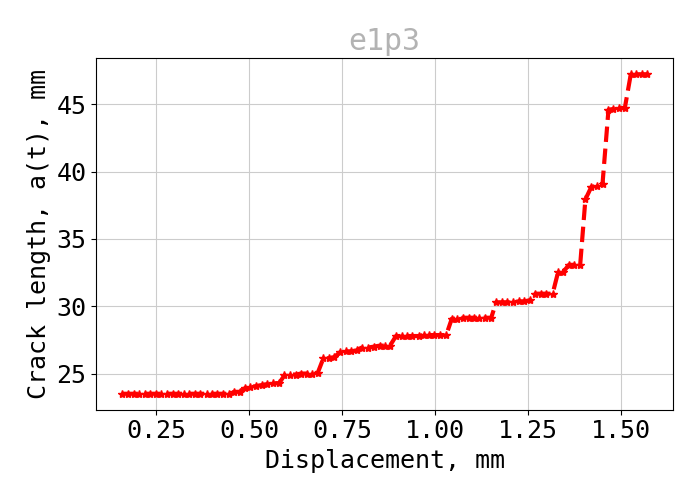
\includegraphics[width=\textwidth]{Figures/e1p3_a}
		\decoRule
		\caption[Crack length E1P3]{Crack length depending on the press displacements, for E1P3 specimen.}
		\label{fig:E1P3_a}
	\end{subfigure}
	\caption{Crack length evolution on Padouck specimens submitted at room climatical conditions and at an average of 5\% moisture content}
	\label{E1p_a}
\end{figure}

\subsection{Energy release rate}

\begin{figure}[H]
\centering
\begin{subfigure}{0.48\linewidth}
	\centering
	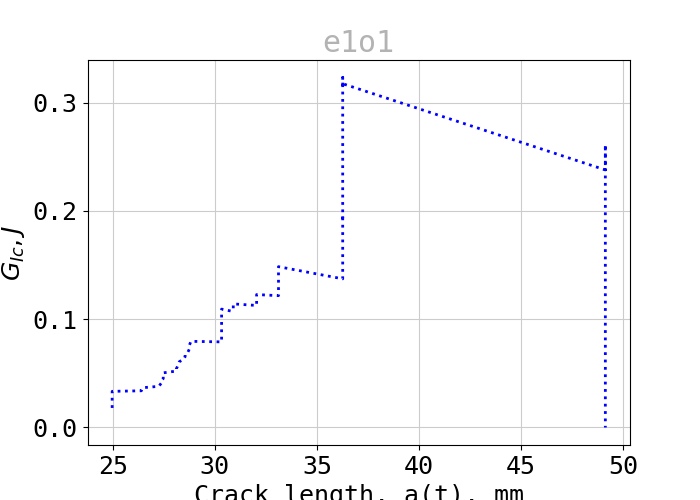
\includegraphics[scale=0.3]{Figures/e1o1_G}
	\decoRule
	\caption[Energy release rate E1O1]{Energy release rate depending on the crack length propagation, for E1O1 specimen.}
	\label{fig:E1O1_G}
\end{subfigure}
\hfill\\
\begin{subfigure}{0.48\linewidth}
	\centering
	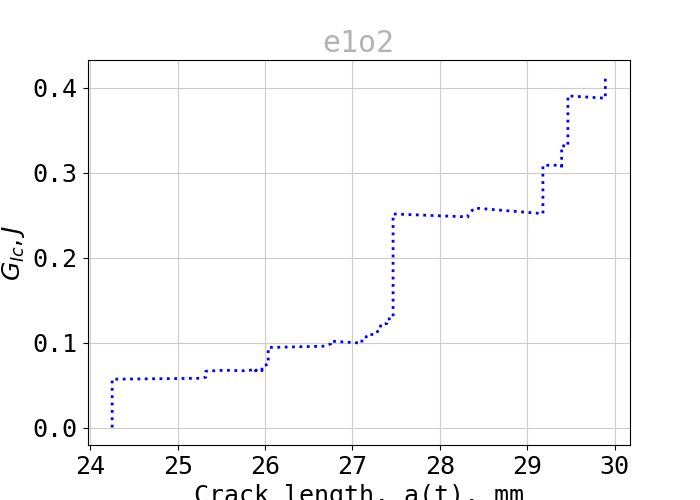
\includegraphics[scale=0.3]{Figures/e1o2_G}
	\decoRule
	\caption[Energy release rate E1O2]{Energy release rate depending on the crack length propagation, for E1O2 specimen.}
	\label{fig:E1O2_G}
\end{subfigure}
\hfill\\
\begin{subfigure}{0.48\linewidth}
	\centering
	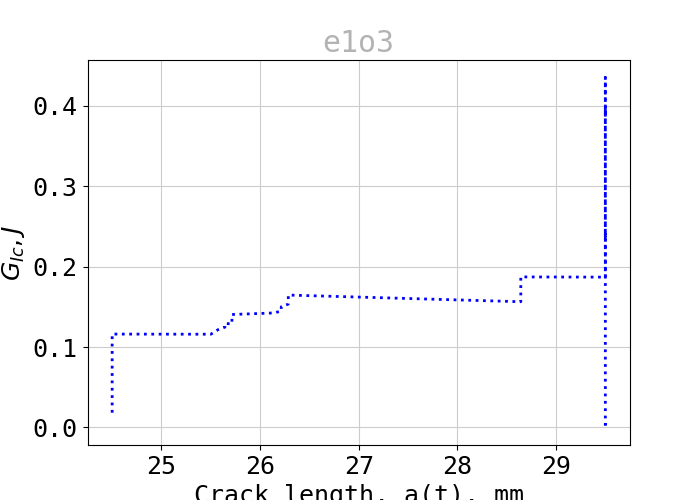
\includegraphics[scale=0.3]{Figures/e1o3_G}
	\decoRule
	\caption[Energy release rate E1O3]{Energy release rate depending on the crack length propagation, for E1O3 specimen.}
	\label{fig:E1O3_G}
\end{subfigure}
\caption{Energy release rate evolution on Okoume specimens at an average of 7\% moisture content}
\label{E1o_G}
\end{figure}

\begin{figure}[H]
\centering
\begin{subfigure}{0.48\linewidth}
	\centering
	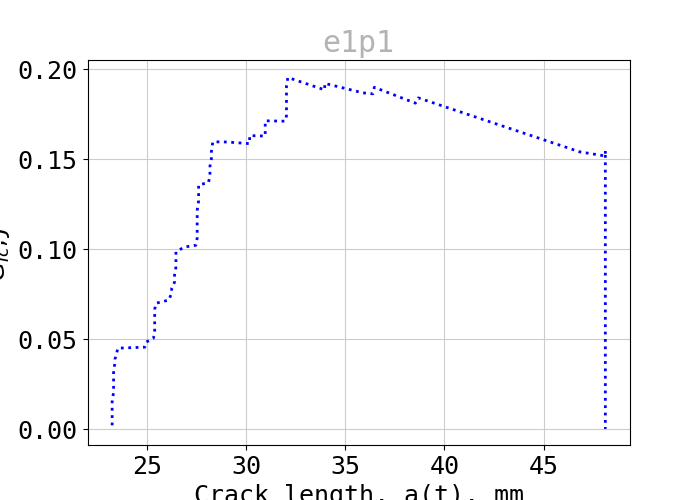
\includegraphics[scale=0.3]{Figures/e1p1_G}
	\decoRule
	\caption[Energy release rate E1P1]{Energy release rate depending on the crack length propagation, for E1P1 specimen.}
	\label{fig:E1P1_G}
\end{subfigure}
\hfill\\
\begin{subfigure}{0.48\linewidth}
	\centering
	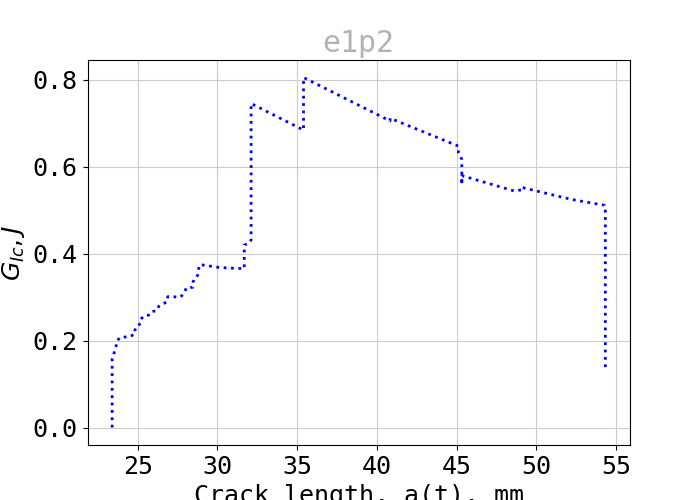
\includegraphics[scale=0.3]{Figures/e1p2_G}
	\decoRule
	\caption[Energy release rate E1P2]{Energy release rate depending on the crack length propagation, for E1P2 specimen.}
	\label{fig:E1P2_G}
\end{subfigure}
\hfill\\
\begin{subfigure}{0.48\linewidth}
	\centering
	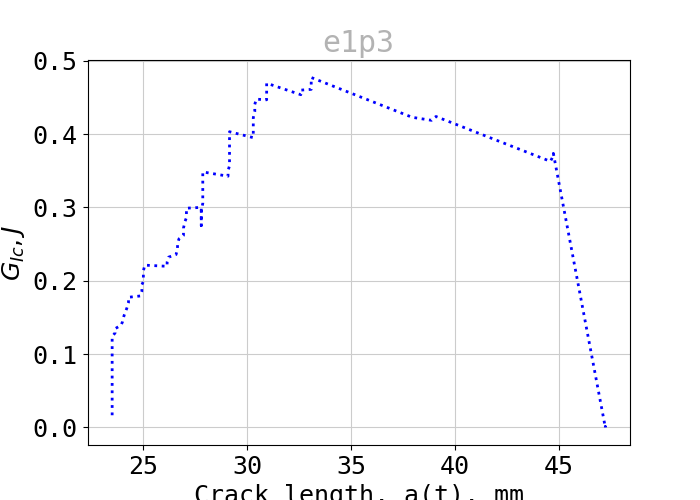
\includegraphics[scale=0.3]{Figures/e1p3_G}
	\decoRule
	\caption[Crack length E1P3]{Crack length depending on the press displacements, for E1P3 specimen.}
	\label{fig:E1P3_G}
\end{subfigure}
\caption{Energy release rate evolution on Padouck specimens at an average of 5\% moisture content}
\label{E1p_G}
\end{figure}
\newpage
\subsection{Cohesive law}

\begin{figure}[H]
	\centering
	\begin{subfigure}{0.48\linewidth}
		\centering
		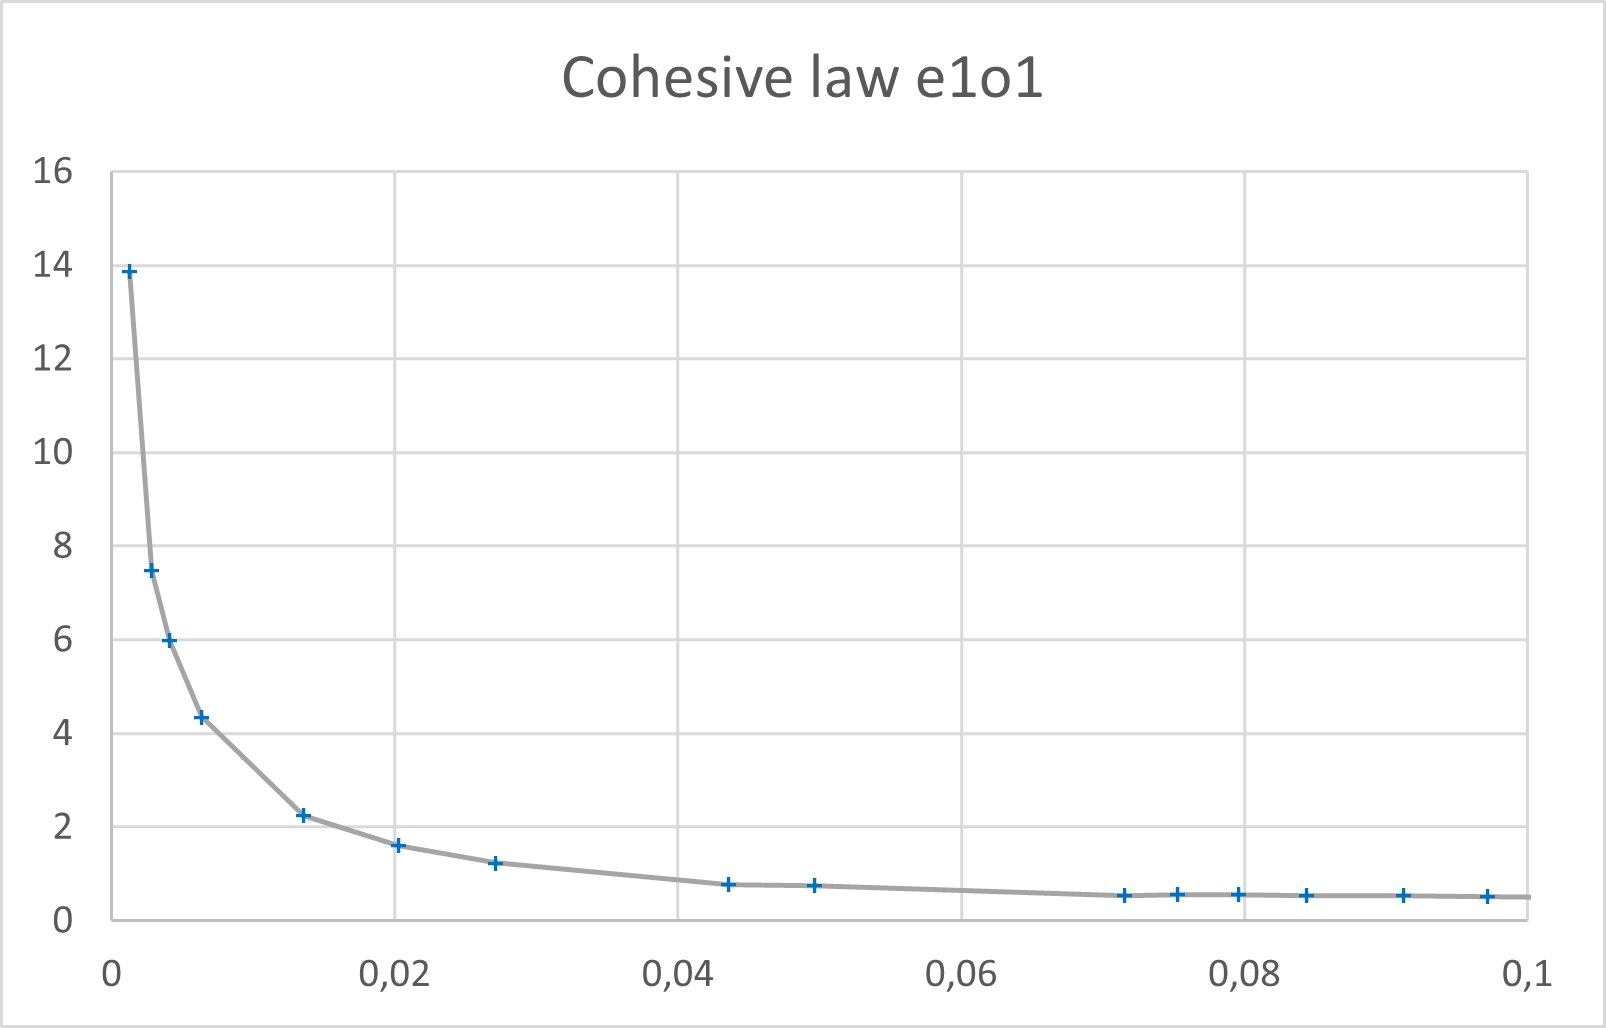
\includegraphics[scale=0.6]{Figures/e1o1_colaw}
		\decoRule
		\caption[Cohesive law from E1O1 specimen]{Cohesive law depending on the crack tip opening displacement and the energy release rate, for E1O1 specimen.}
		\label{fig:E1O1_colaw}
	\end{subfigure}
	\hfill\\
	\begin{subfigure}{0.48\linewidth}
		\centering
		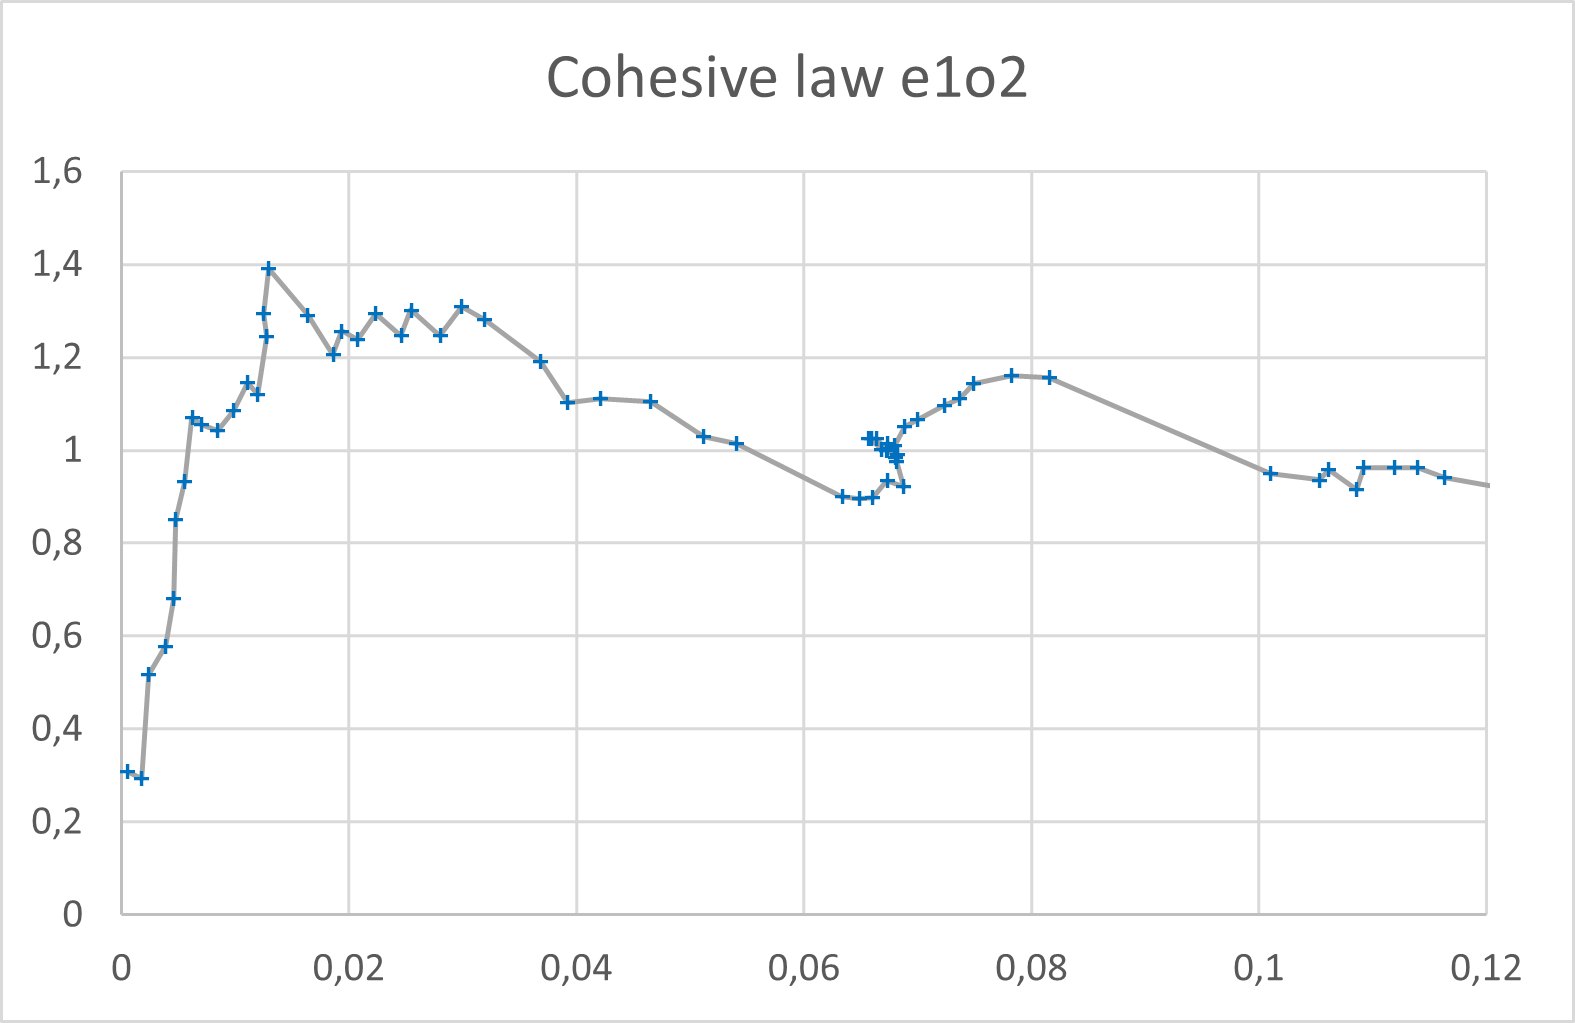
\includegraphics[scale=0.6]{Figures/e1o2_colaw}
		\decoRule
		\caption[Cohesive law from E1O2 specimen]{Cohesive law depending on the crack tip opening displacement and the energy release rate, for E1O2 specimen.}
		\label{fig:E1O2_colaw}
	\end{subfigure}
	\hfill\\
	\begin{subfigure}{0.48\linewidth}
		\centering
		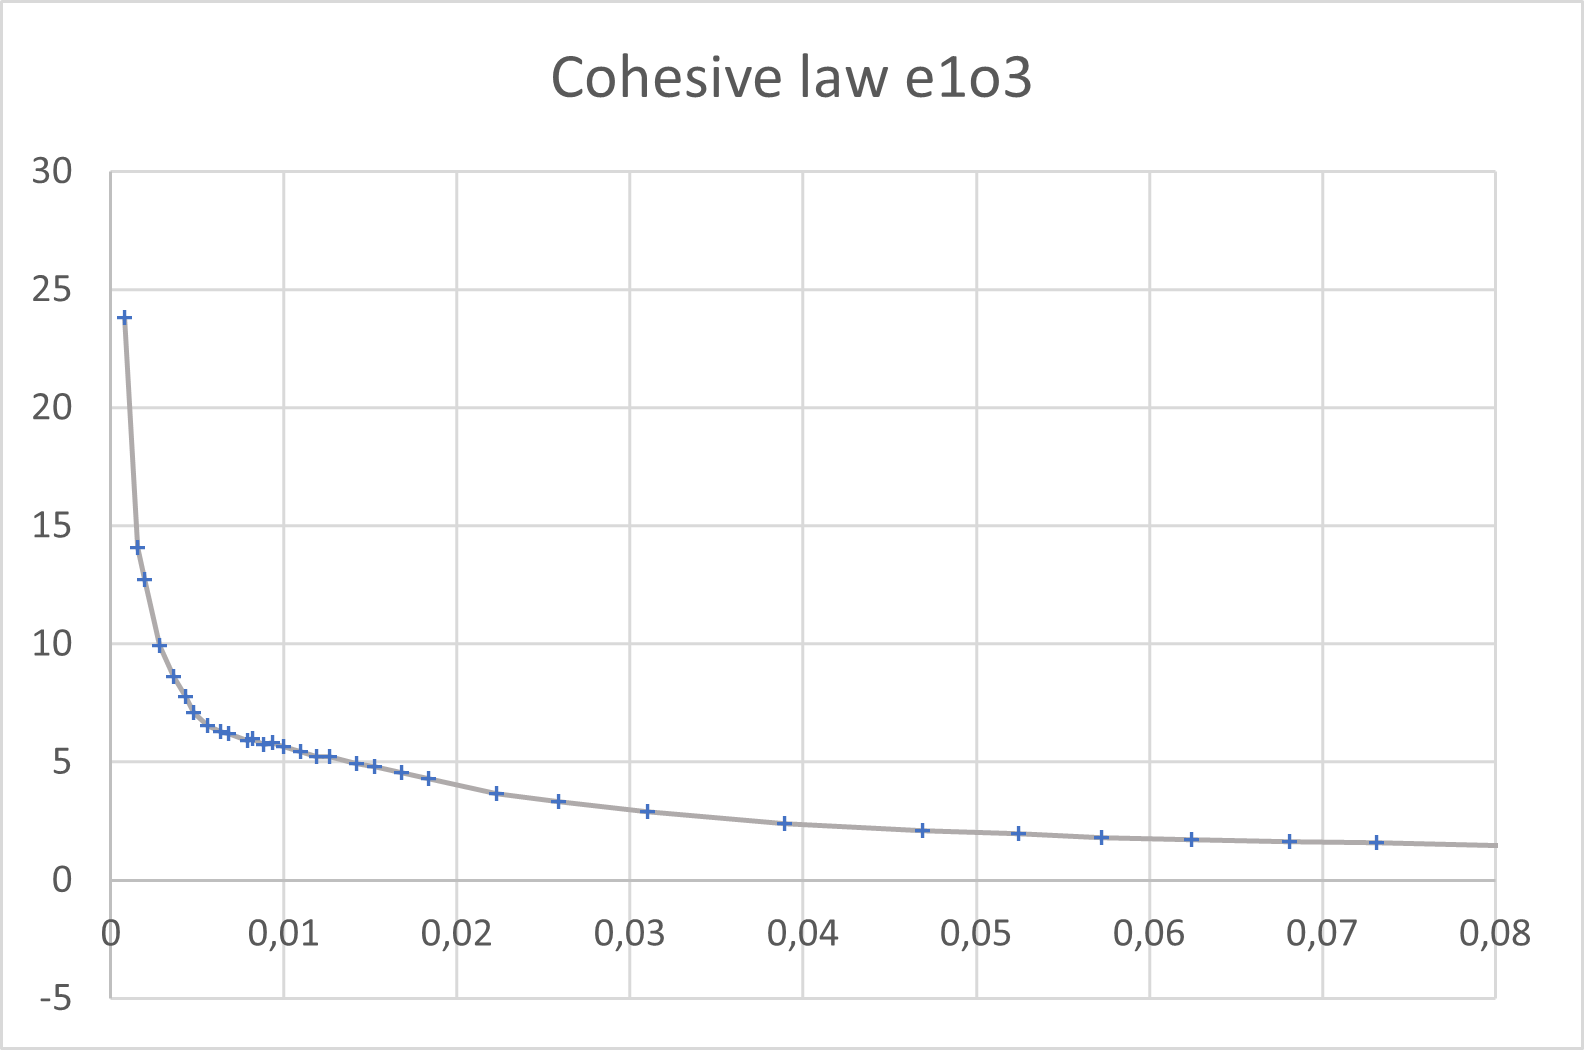
\includegraphics[scale=0.6]{Figures/e1o3_colaw}
		\decoRule
		\caption[Cohesive law from E1O3 specimen]{Cohesive law depending on the crack tip opening displacement and the energy release rate, for E1O3 specimen.}
		\label{fig:E1O3_colaw}
	\end{subfigure}
	\caption{Cohesive law from Okoume specimens at an average of 7\% moisture content}
	\label{E1o_colaw}
\end{figure}

\begin{figure}[H]
	\centering
	\begin{subfigure}{0.48\linewidth}
		\centering
		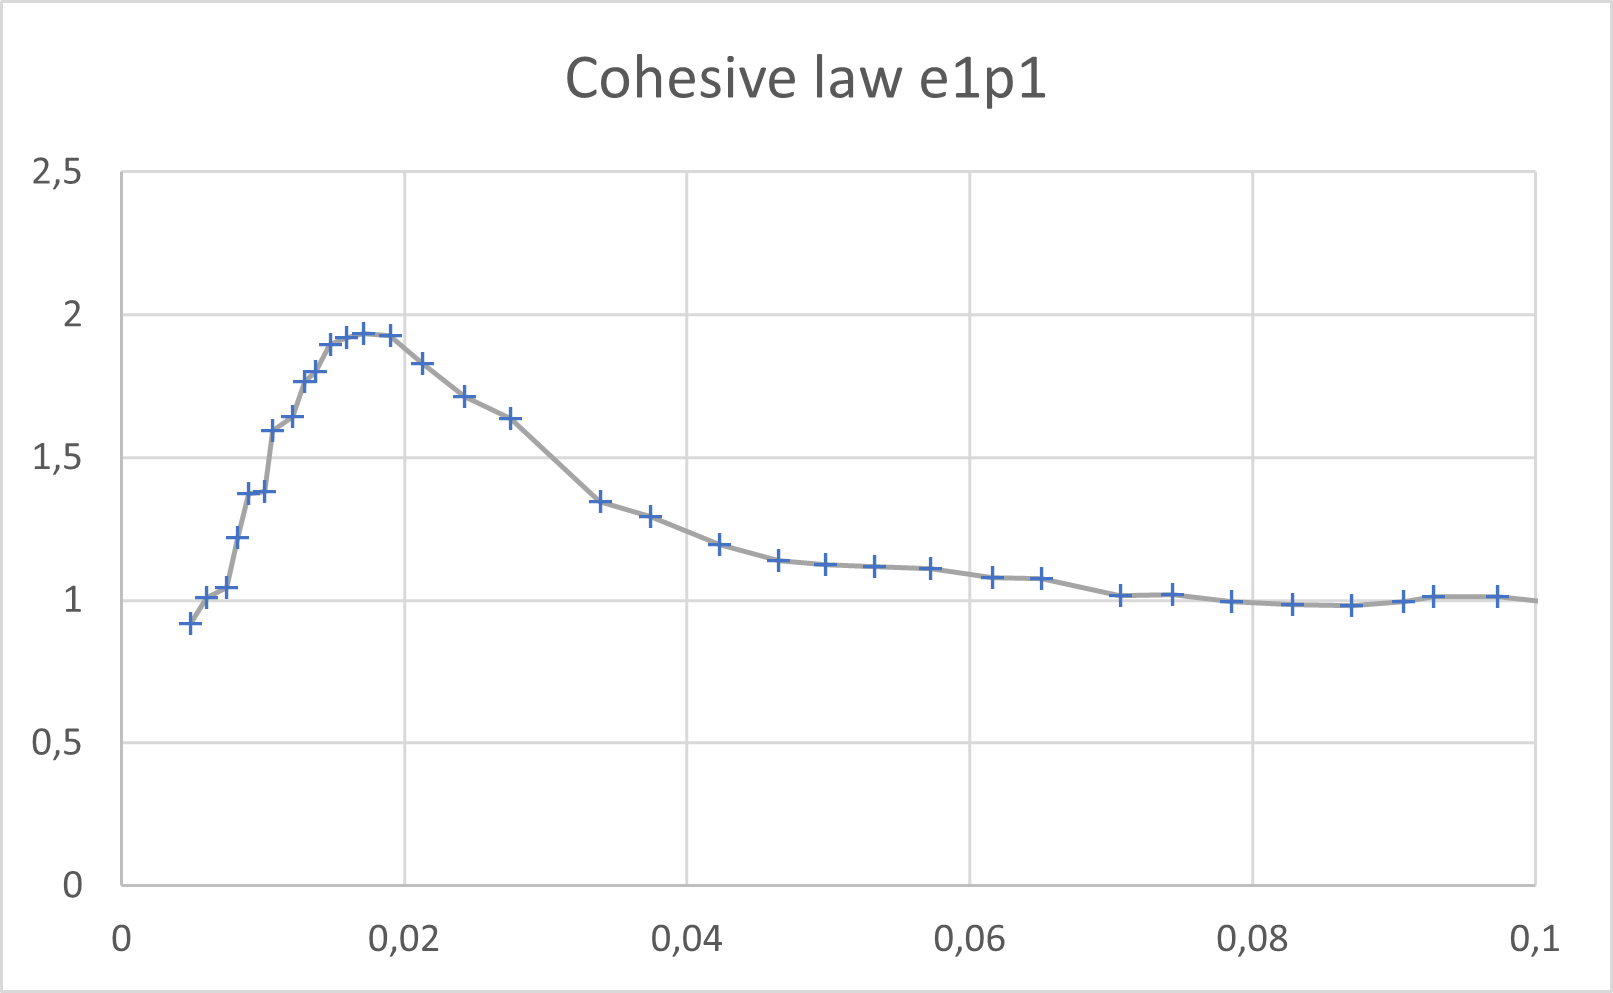
\includegraphics[scale=0.6]{Figures/e1p1_colaw}
		\decoRule
		\caption[Cohesive law from E1P1 specimen]{Cohesive law depending on the crack tip opening displacement and the energy release rate, for E1P1 specimen.}
		\label{fig:E1P1_colaw}
	\end{subfigure}
	\hfill\\
	\begin{subfigure}{0.48\linewidth}
		\centering
		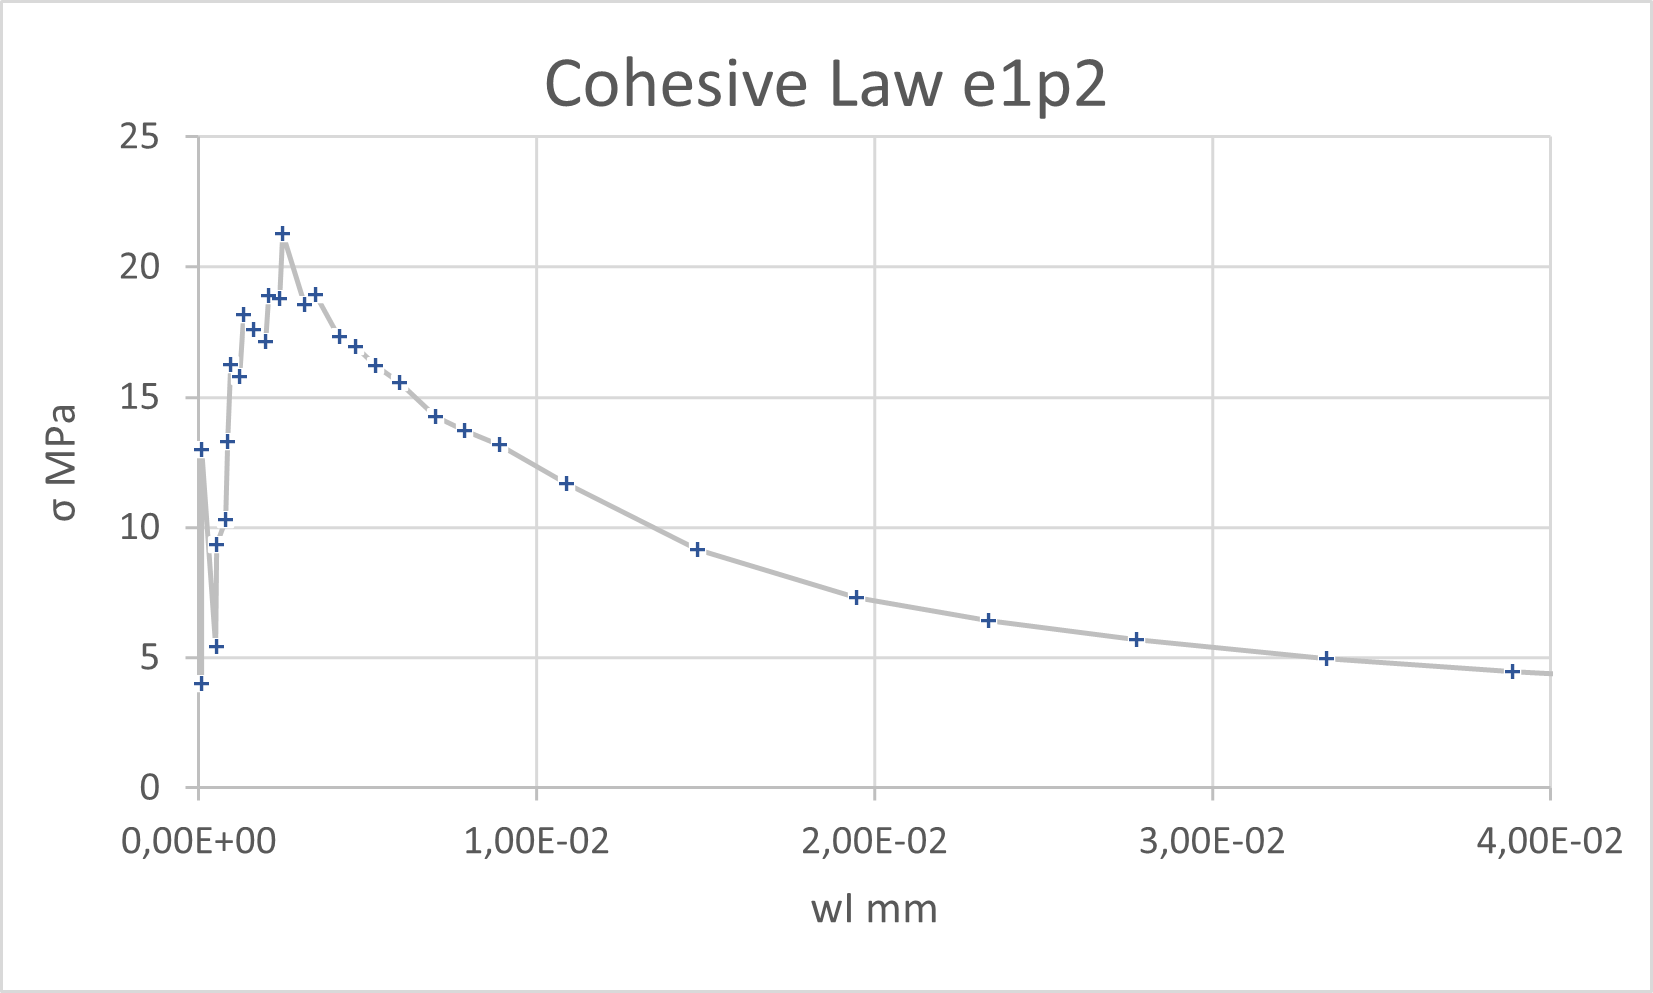
\includegraphics[scale=0.6]{Figures/e1p2_colaw}
		\decoRule
		\caption[Cohesive law from E1P2 specimen]{Cohesive law depending on the crack tip opening displacement and the energy release rate, for E1P2 specimen.}
		\label{fig:E1P2_colaw}
	\end{subfigure}
	\hfill\\
	\begin{subfigure}{0.48\linewidth}
		\centering
		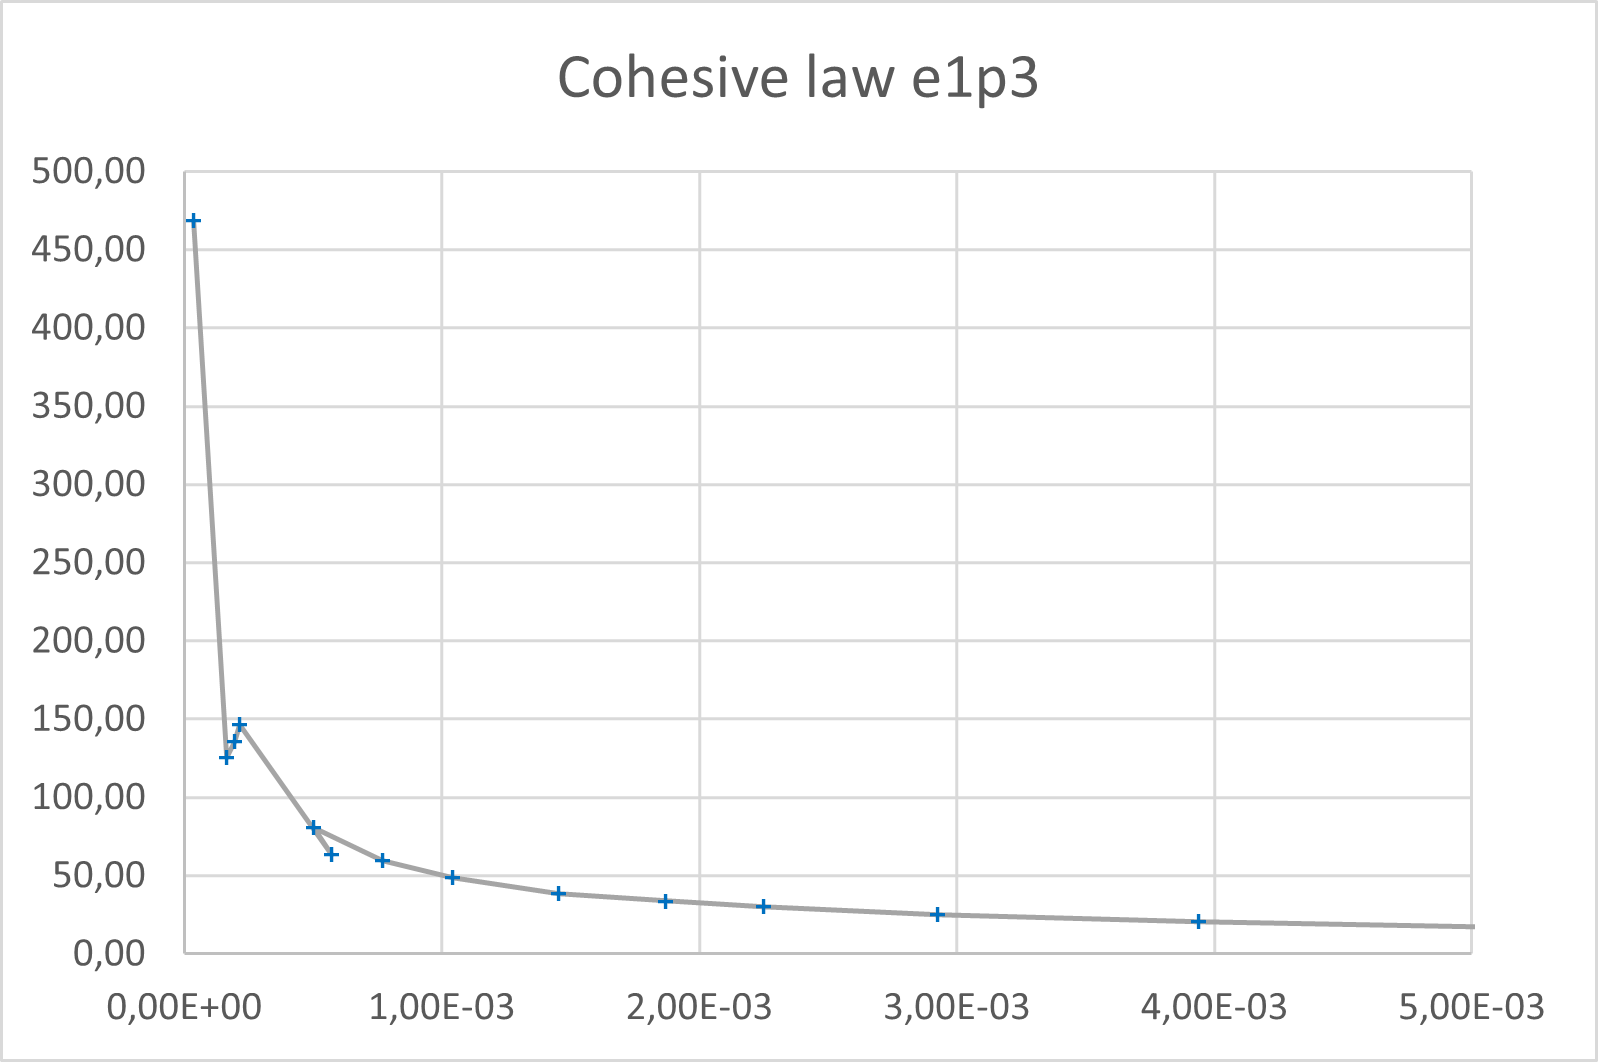
\includegraphics[scale=0.6]{Figures/e1p3_colaw}
		\decoRule
		\caption[Cohesive law from E1P3 specimen]{Cohesive law depending on the crack tip opening displacement and the energy release rate, for E1P3 specimen.}
		\label{fig:E1P3_colaw}
	\end{subfigure}
	\caption{Cohesive law from Okoume specimens at an average of 5\% moisture content}
	\label{E1p_colaw}
\end{figure}
\newpage
%%%%%%%%%%%%%%%%%%%%%%%%%%%%%%%%%%%%%%%%%%%%%%%%%
%Section 2
%%%%%%%%%%%%%%%%%%%%%%%%%%%%%%%%%%%%%%%%%%%%%%%%%

\section{Results at 20\% Moisture Content}

\subsection{Crack length}

\begin{figure}[H]
\centering
\begin{subfigure}{0.48\linewidth}
	\centering
	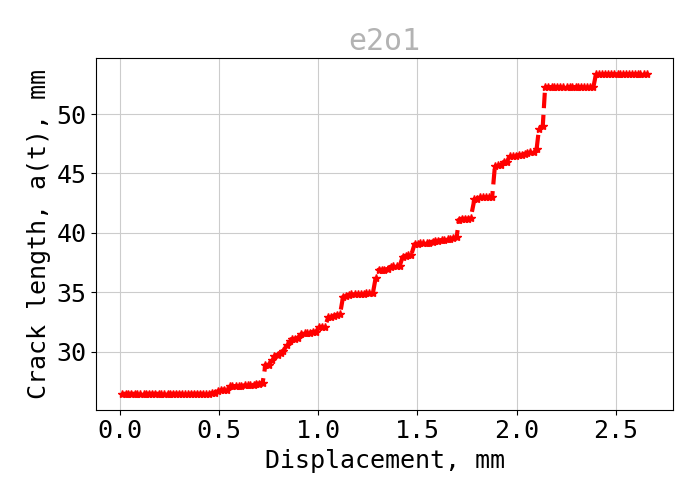
\includegraphics[width=\textwidth]{Figures/e2o1_a}
	\decoRule
	\caption[Crack length E2O1]{Crack length depending on the press displacements, for E2O1 specimen.}
	\label{fig:E2O1_a}
\end{subfigure}
\hfill\\
\begin{subfigure}{0.48\linewidth}
	\centering
	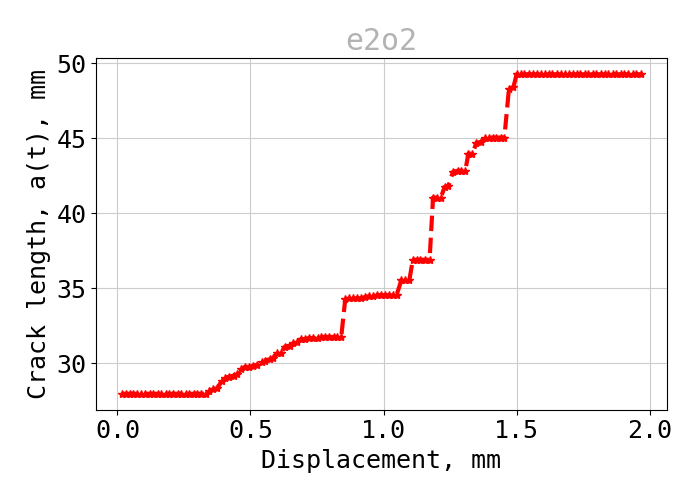
\includegraphics[width=\textwidth]{Figures/e2o2_a}
	\decoRule
	\caption[Crack length E2O2]{Crack length depending on the press displacements, for E2O2 specimen.}
	\label{fig:E2O2_a}
\end{subfigure}
\hfill\\
\begin{subfigure}{0.48\linewidth}
	\centering
	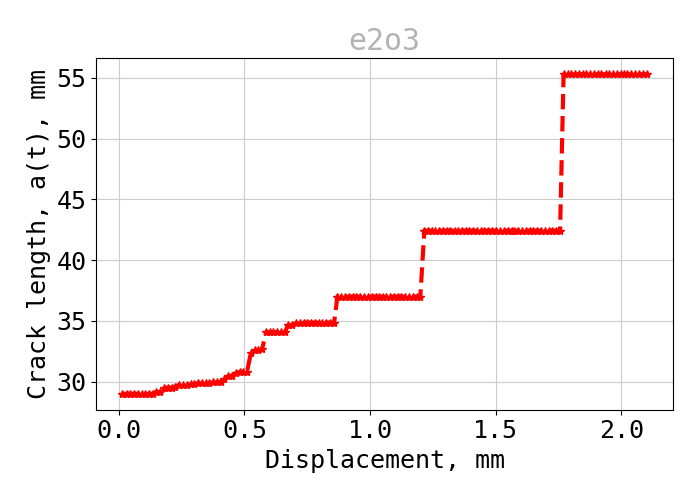
\includegraphics[width=\textwidth]{Figures/e2o3_a}
	\decoRule
	\caption[Crack length E2O3]{Crack length depending on the press displacements, for E2O3 specimen.}
	\label{fig:E2O3_a}
\end{subfigure}
\caption{Crack length evolution on Okoume specimens at an average of 19\% moisture content}
\label{E2o_a}
\end{figure}

\begin{figure}[H]
\centering
\begin{subfigure}{0.48\linewidth}
	\centering
	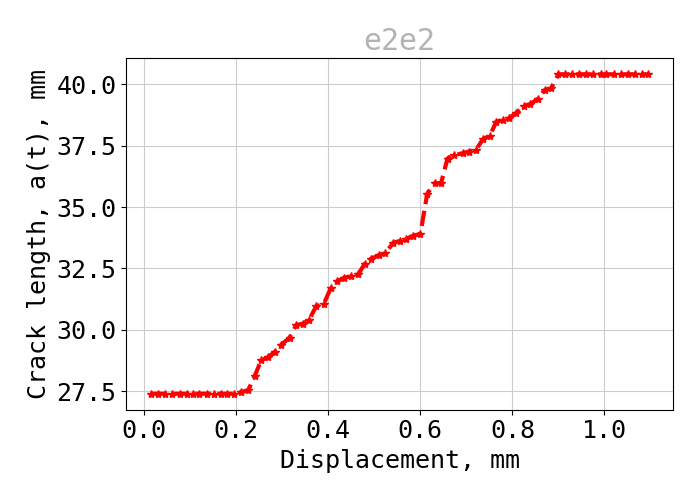
\includegraphics[scale=0.3]{Figures/e2p1_a}
	\decoRule
	\caption[Crack length E2P1]{Crack length depending on the press displacements, for E2P1 specimen.}
	\label{fig:E2P1_a}
\end{subfigure}
\hfill\\
\begin{subfigure}{0.48\linewidth}
	\centering
	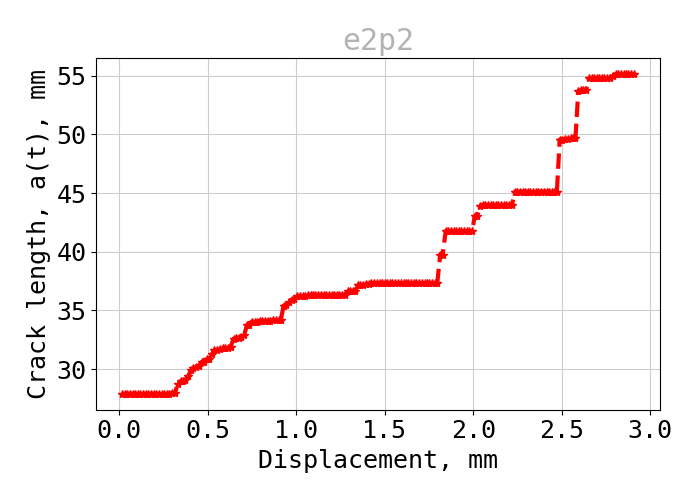
\includegraphics[scale=0.3]{Figures/e2p2_a}
	\decoRule
	\caption[Crack length E2P2]{Crack length depending on the press displacements, for E2P2 specimen.}
	\label{fig:E2P2_a}
\end{subfigure}
\hfill\\
\begin{subfigure}{0.48\linewidth}
	\centering
	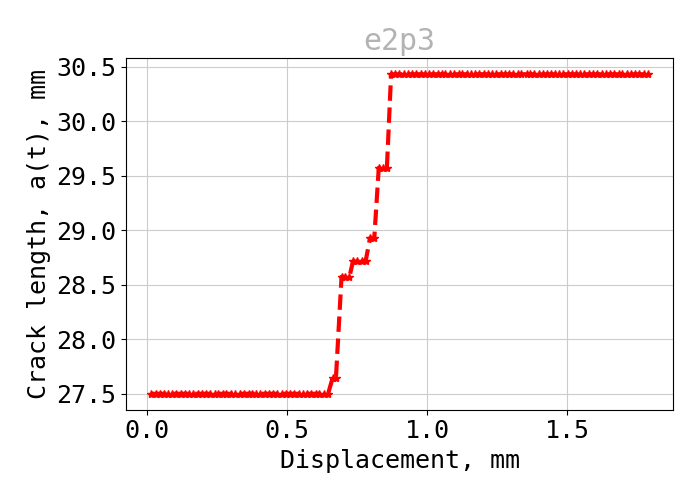
\includegraphics[scale=0.3]{Figures/e2p3_a}
	\decoRule
	\caption[Crack length E2P3]{Crack length depending on the press displacements, for E2P3 specimen.}
	\label{fig:E2P3_a}
\end{subfigure}
\caption{Crack length evolution on Padouck specimens at an average of 15\% moisture content}
\label{E2p_a}
\end{figure}
\newpage
\subsection{Energy release rate}

\begin{figure}[H]
\centering
\begin{subfigure}{0.48\linewidth}
	\centering
	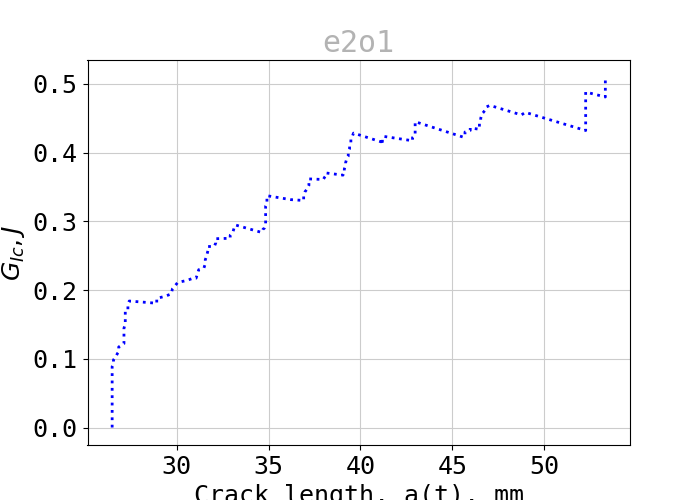
\includegraphics[scale=0.3]{Figures/e2o1_G}
	\decoRule
	\caption[Energy release rate E2O1]{Energy release rate depending on the crack length propagation, for E2O1 specimen.}
	\label{fig:E2O1_G}
\end{subfigure}
\hfill\\
\begin{subfigure}{0.48\linewidth}
	\centering
	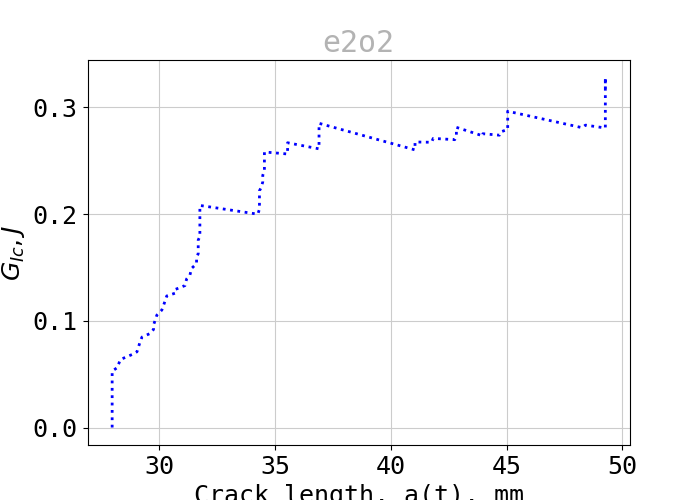
\includegraphics[scale=0.3]{Figures/e2o2_G}
	\decoRule
	\caption[Energy release rate E2O2]{Energy release rate depending on the crack length propagation, for E2O2 specimen.}
	\label{fig:E2O2_G}
\end{subfigure}
\hfill\\
\begin{subfigure}{0.48\linewidth}
	\centering
	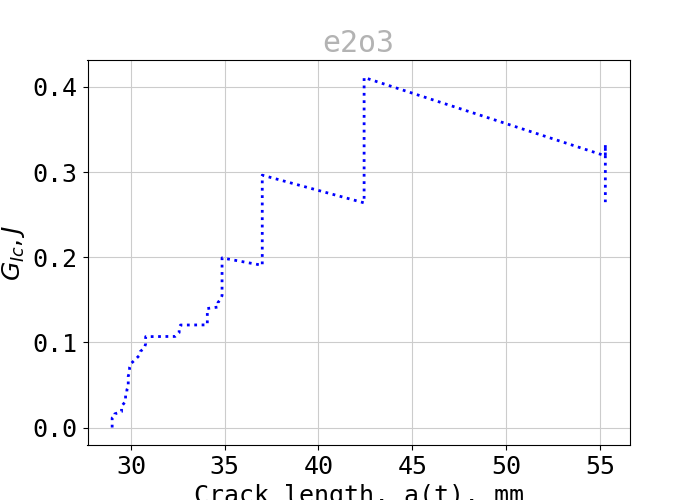
\includegraphics[scale=0.3]{Figures/e2o3_G}
	\decoRule
	\caption[Energy release rate E2O3]{Energy release rate depending on the crack length propagation, for E2O3 specimen.}
	\label{fig:E2O3_G}
\end{subfigure}
\caption{Energy release rate evolution on Okoume specimens at an average of 19\% moisture content}
\label{E2o_G}
\end{figure}

\newpage
\begin{figure}[H]
\centering
\begin{subfigure}{0.48\linewidth}
	\centering
	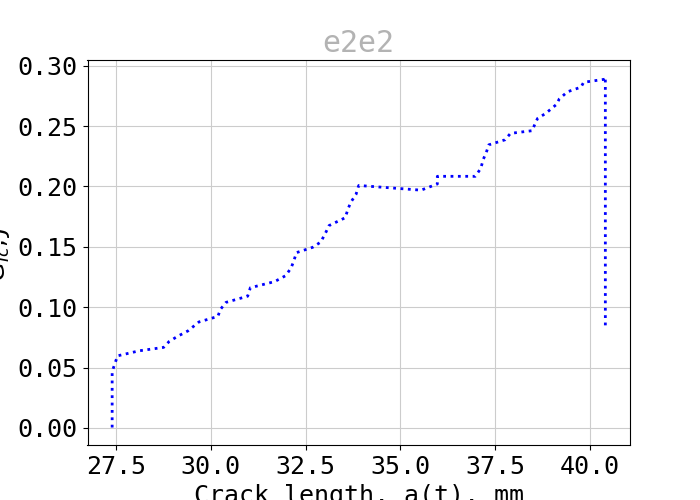
\includegraphics[scale=0.3]{Figures/e2p1_G}
	\decoRule
	\caption[Energy release rate E2P1]{Energy release rate depending on the crack length propagation, for E2P1 specimen.}
	\label{fig:E2P1_G}
\end{subfigure}
\hfill\\
\begin{subfigure}{0.48\linewidth}
	\centering
	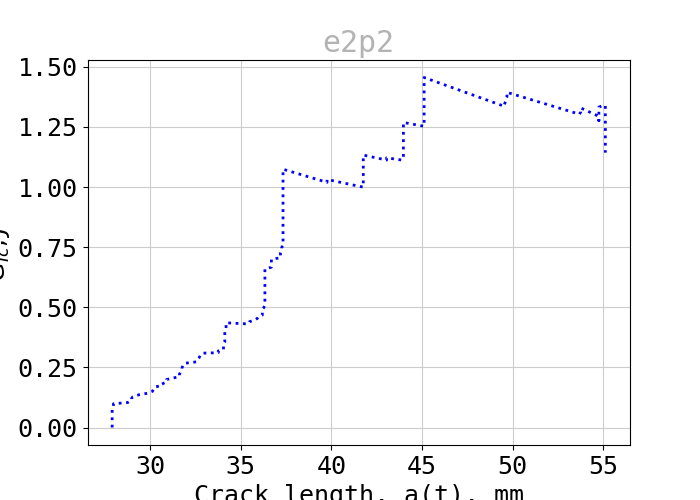
\includegraphics[scale=0.3]{Figures/e2p2_G}
	\decoRule
	\caption[Energy release rate E2P2]{Energy release rate depending on the crack length propagation, for E2P2 specimen.}
	\label{fig:E2P2_G}
\end{subfigure}
\hfill\\
\begin{subfigure}{0.48\linewidth}
	\centering
	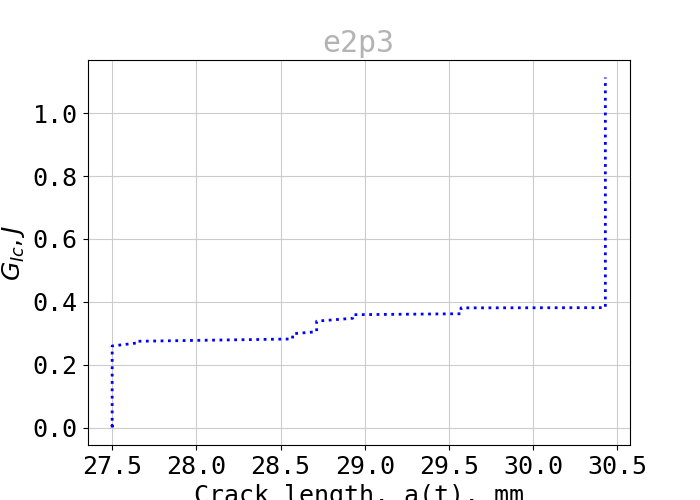
\includegraphics[scale=0.3]{Figures/e2p3_G}
	\decoRule
	\caption[Crack length E2P3]{Crack length depending on the press displacements, for E2P3 specimen.}
	\label{fig:E2P3_G}
\end{subfigure}
\caption{Energy release rate evolution on Padouck specimens at an average of 15\% moisture content}
\label{E2p_G}
\end{figure}
\newpage
\subsection{Cohesive law}

\begin{figure}[H]
\centering
\begin{subfigure}{0.48\linewidth}
	\centering
	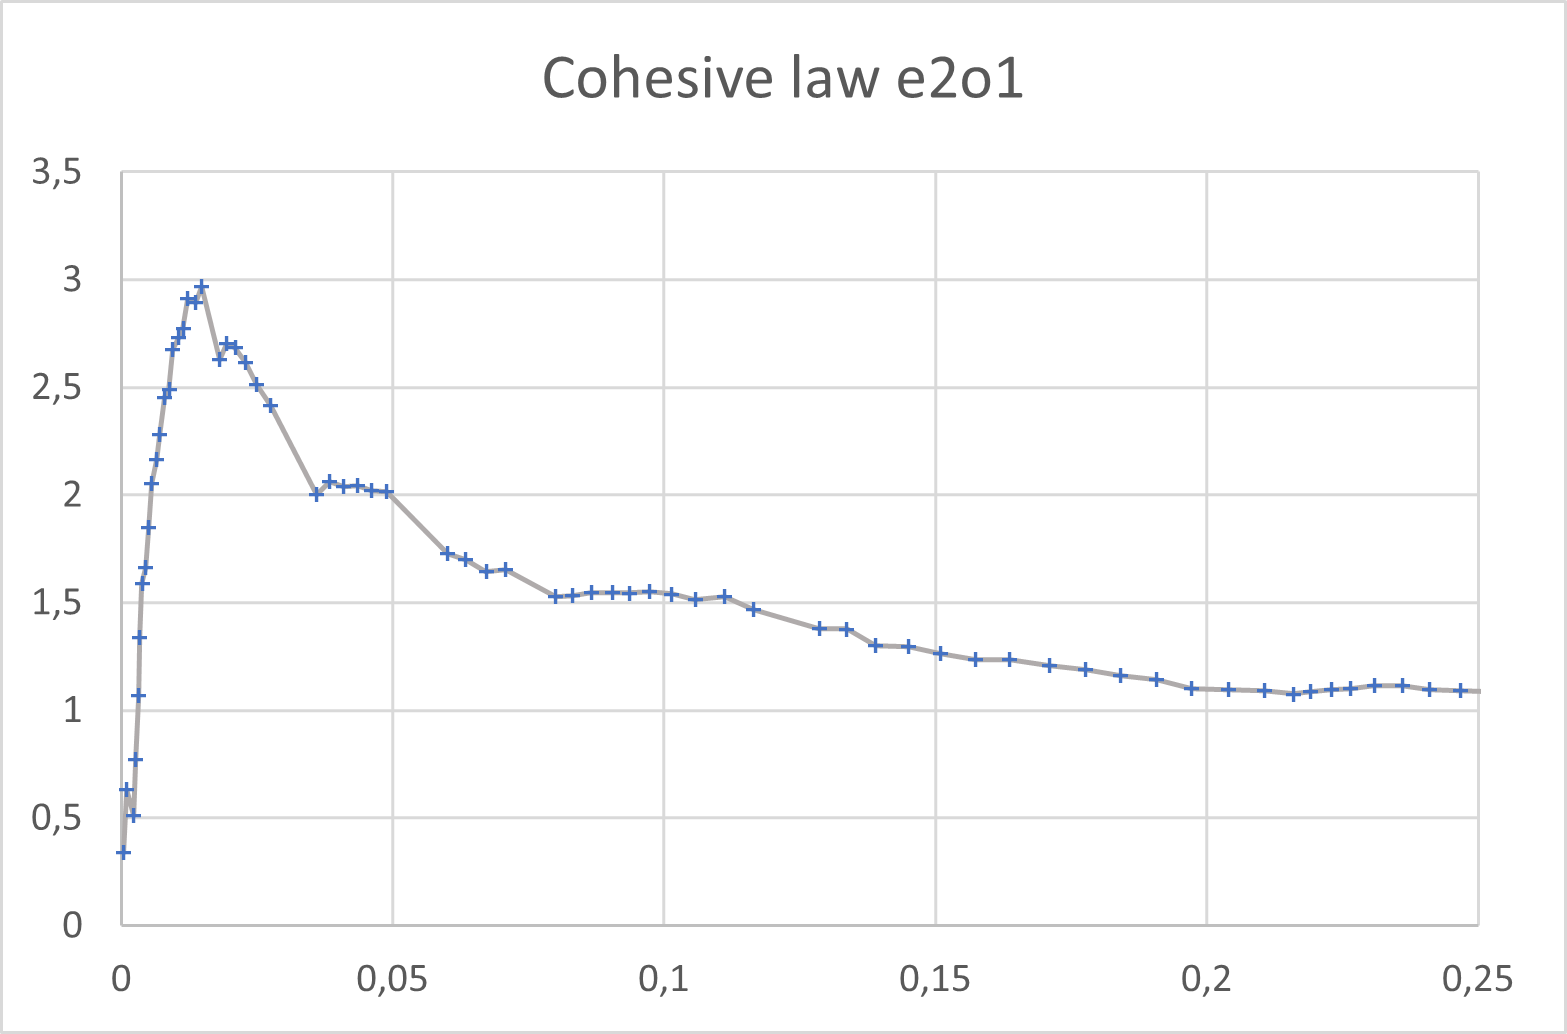
\includegraphics[scale=0.6]{Figures/e2o1_colaw}
	\decoRule
	\caption[Cohesive law from E2O1 specimen]{Cohesive law depending on the crack tip opening displacement and the energy release rate, for E2O1 specimen.}
	\label{fig:E2O1_colaw}
\end{subfigure}
\hfill\\
\begin{subfigure}{0.48\linewidth}
	\centering
	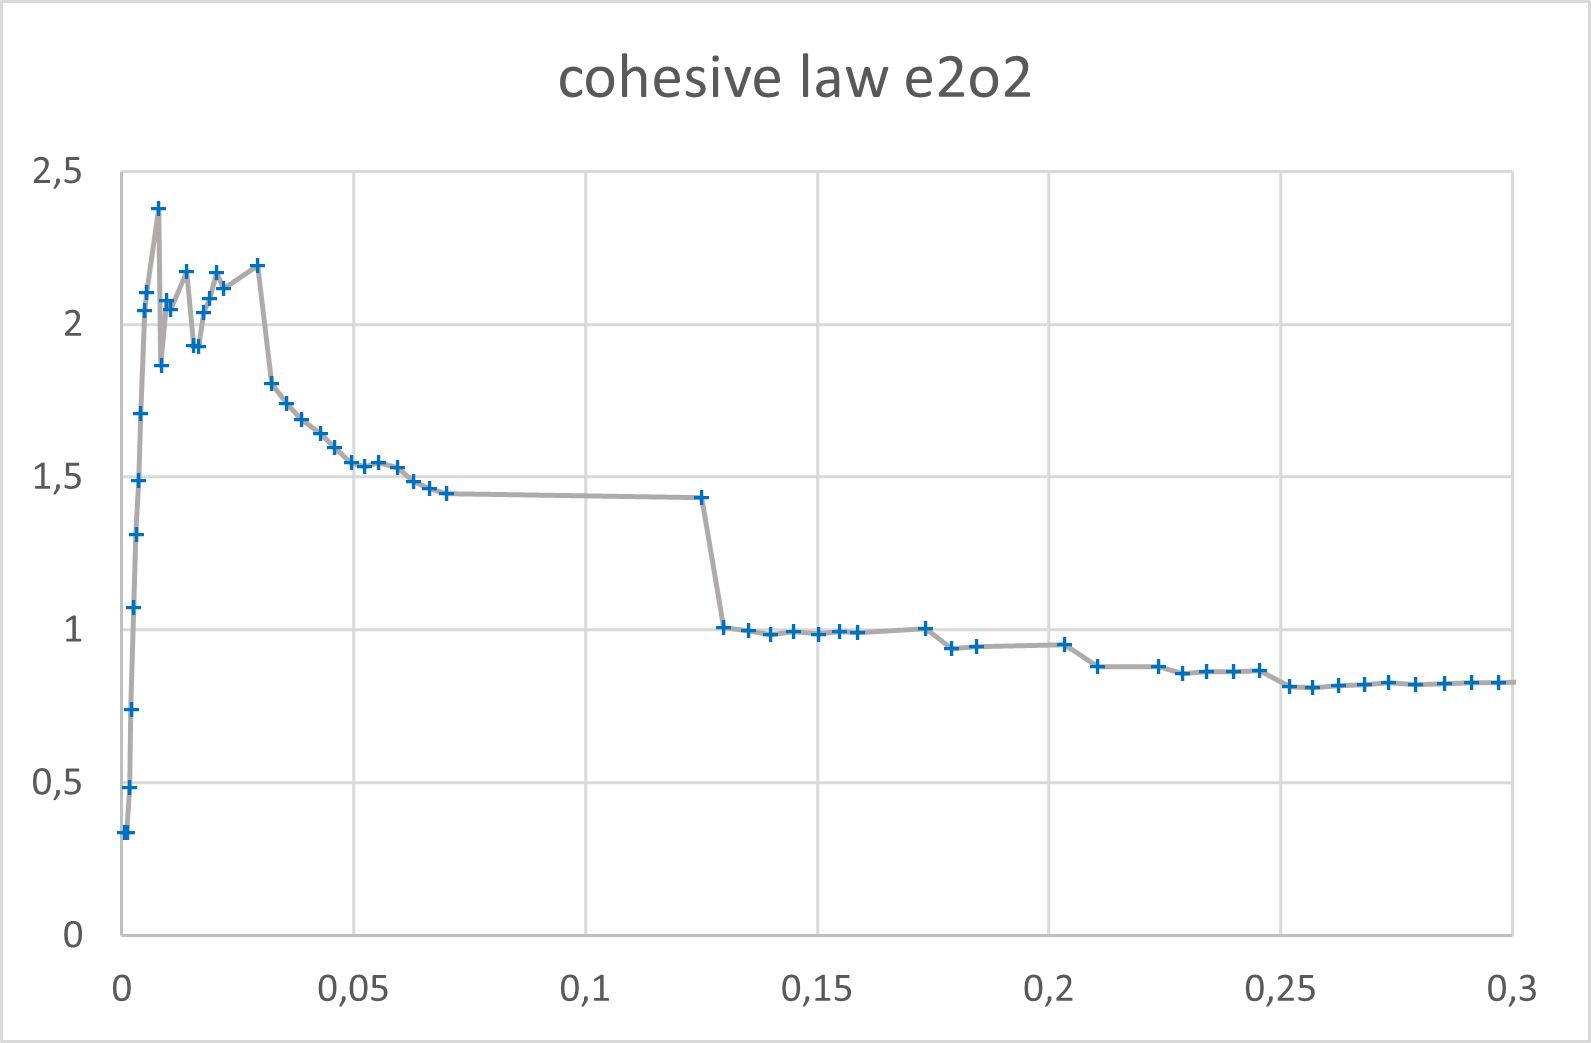
\includegraphics[scale=0.6]{Figures/e2o2_colaw}
	\decoRule
	\caption[Cohesive law from E2O2 specimen]{Cohesive law depending on the crack tip opening displacement and the energy release rate, for E2O2 specimen.}
	\label{fig:E2O2_colaw}
\end{subfigure}
\hfill\\
\begin{subfigure}{0.48\linewidth}
	\centering
	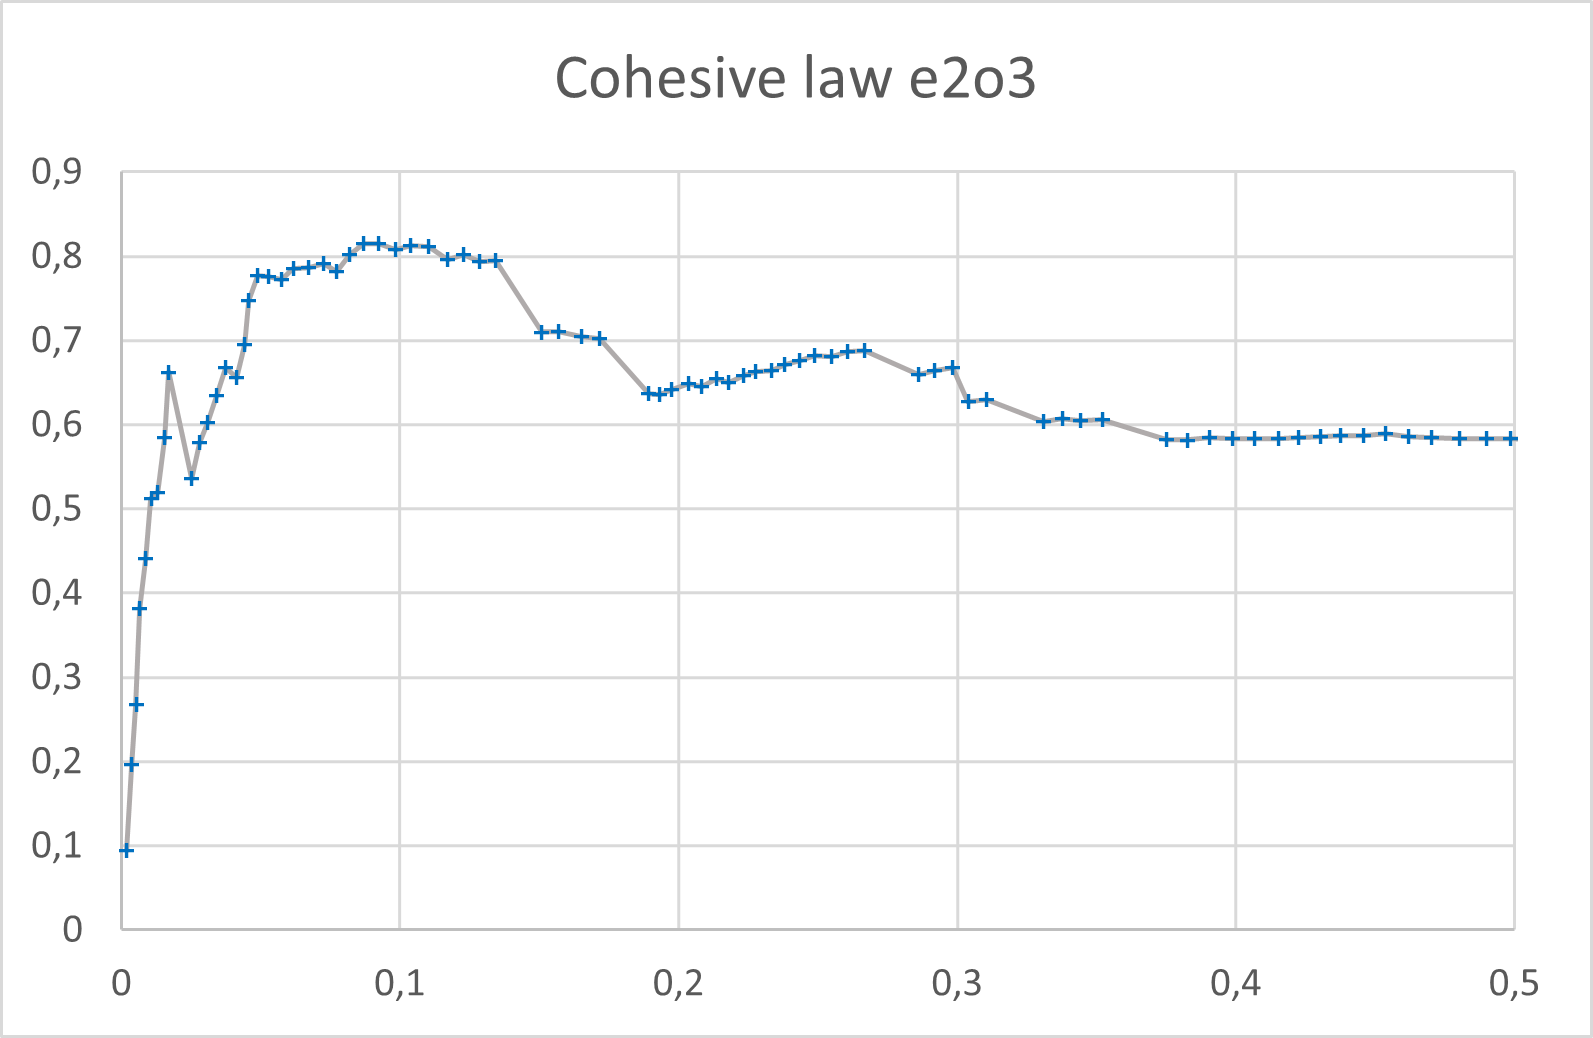
\includegraphics[scale=0.6]{Figures/e2o3_colaw}
	\decoRule
	\caption[Cohesive law from E1O3 specimen]{Cohesive law depending on the crack tip opening displacement and the energy release rate, for E2O3 specimen.}
	\label{fig:E2O3_colaw}
\end{subfigure}
\caption{Cohesive law from Okoume specimens at an average of 19\% moisture content}
\label{E2o_colaw}
\end{figure}
\newpage
\begin{figure}[H]
\centering
\begin{subfigure}{0.48\linewidth}
	\centering
	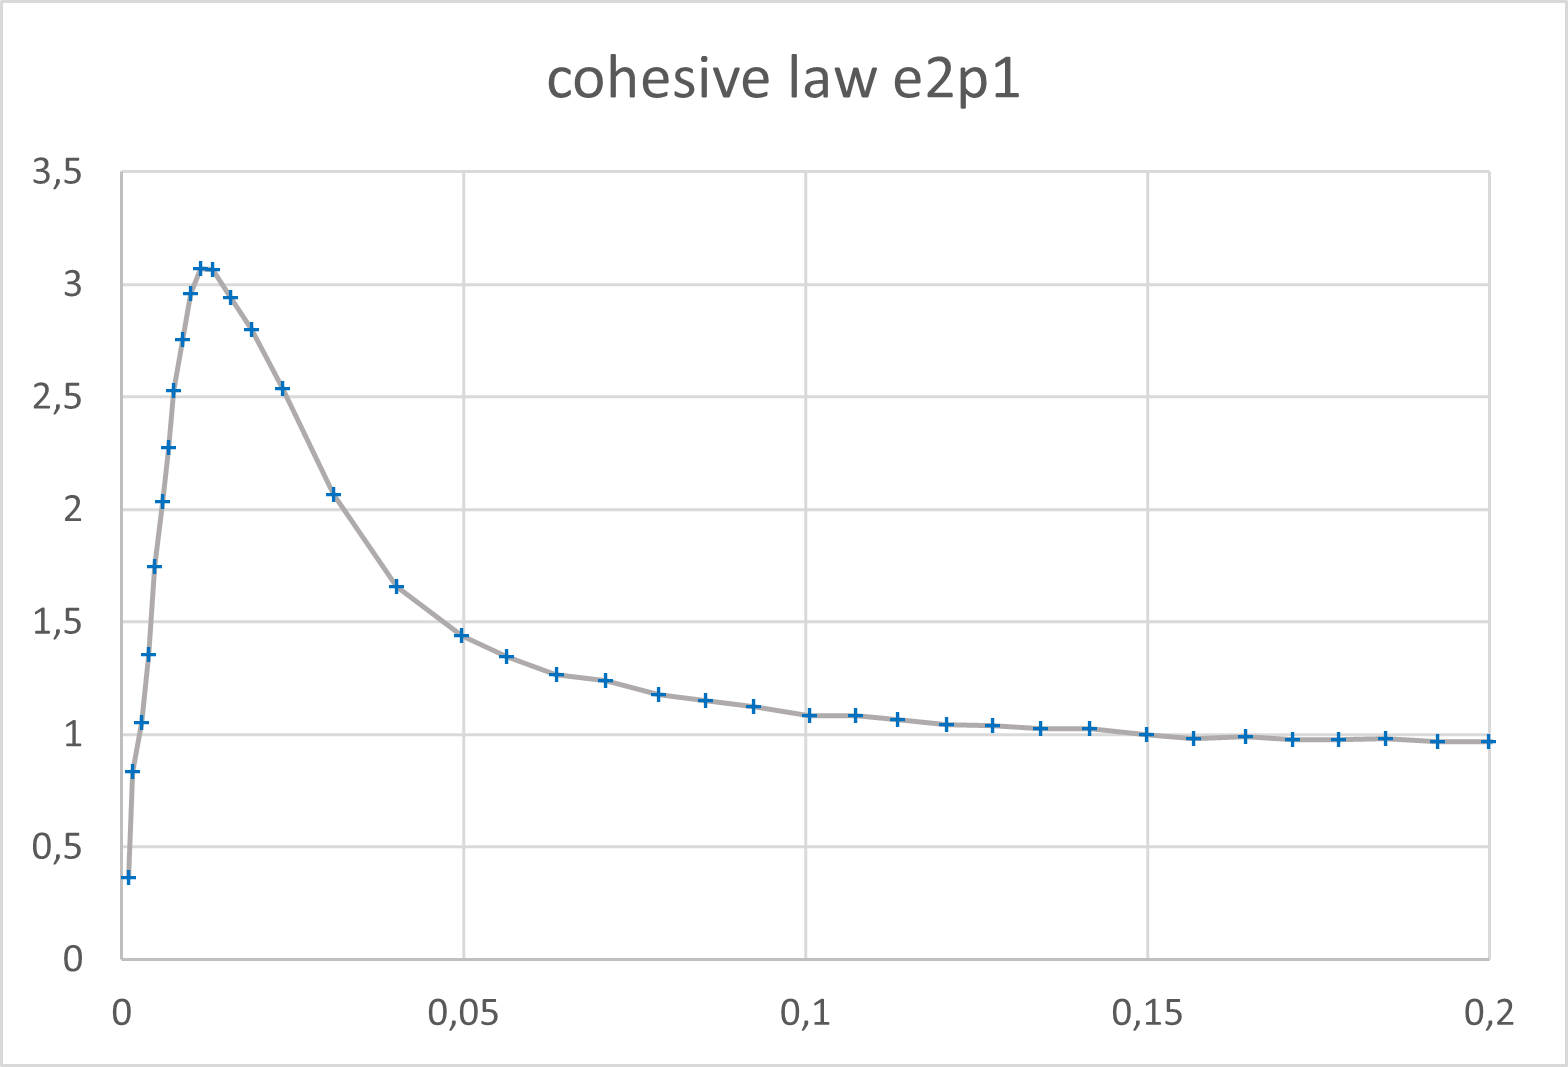
\includegraphics[scale=0.6]{Figures/e2p1_colaw}
	\decoRule
	\caption[Cohesive law from E2P1 specimen]{Cohesive law depending on the crack tip opening displacement and the energy release rate, for E2P1 specimen.}
	\label{fig:E2P1_colaw}
\end{subfigure}
\hfill\\
\begin{subfigure}{0.48\linewidth}
	\centering
	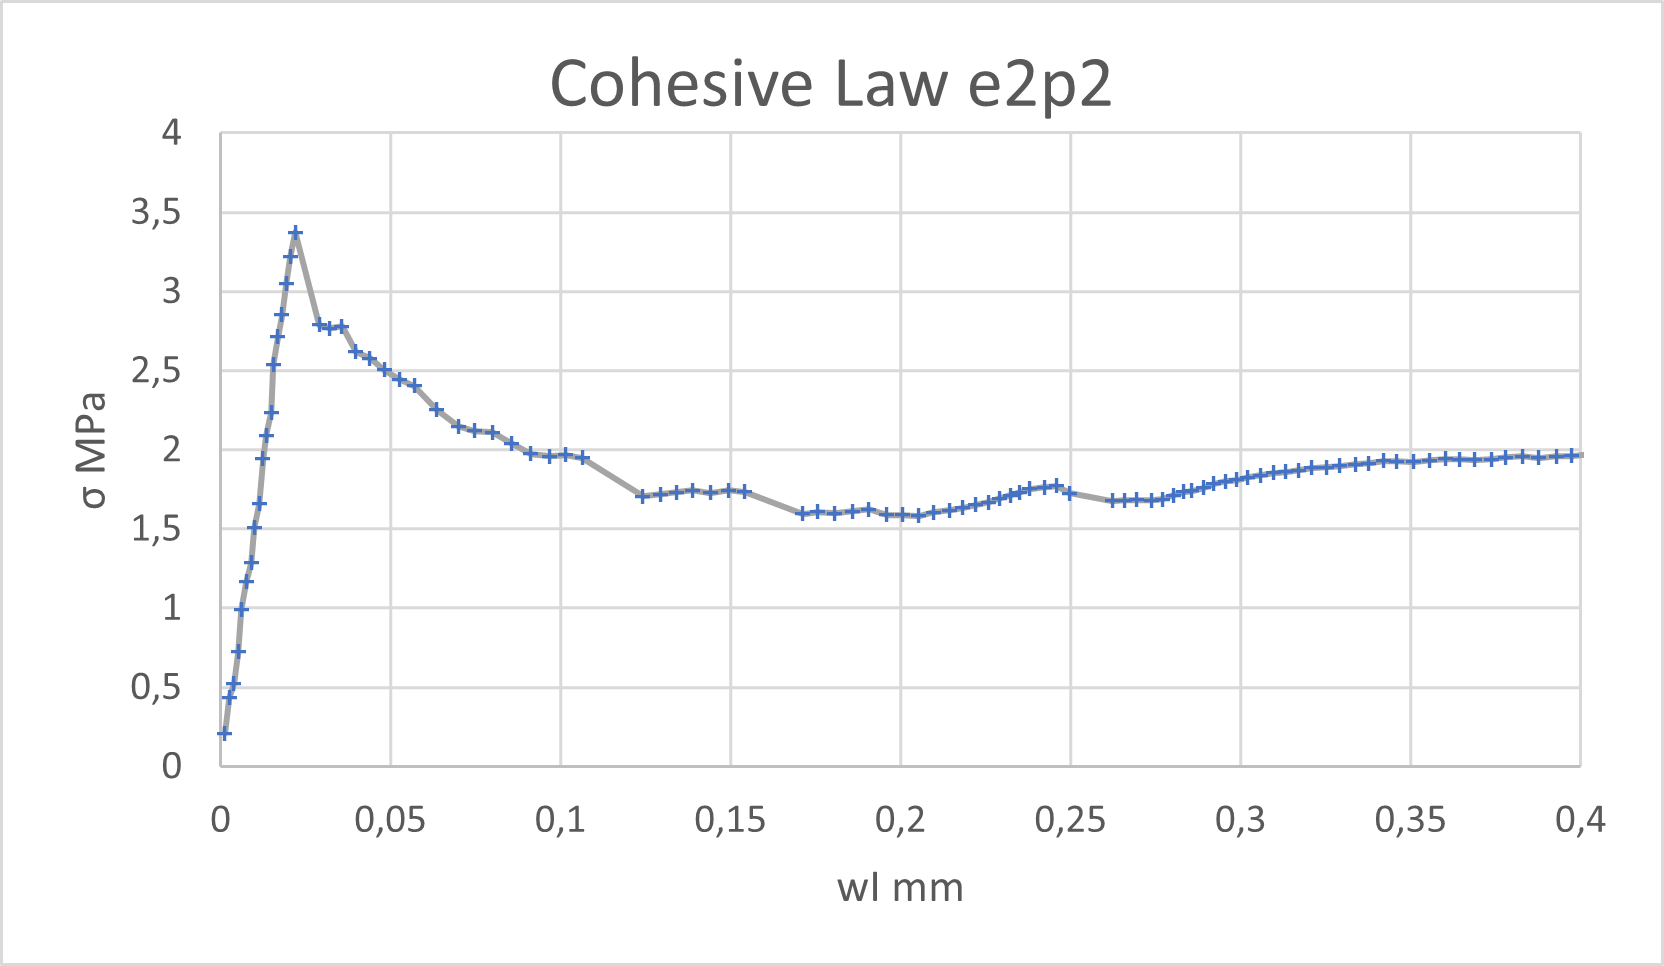
\includegraphics[scale=0.6]{Figures/e2p2_colaw}
	\decoRule
	\caption[Cohesive law from E2P2 specimen]{Cohesive law depending on the crack tip opening displacement and the energy release rate, for E2P2 specimen.}
	\label{fig:E2P2_colaw}
\end{subfigure}
\hfill\\
\begin{subfigure}{0.48\linewidth}
	\centering
	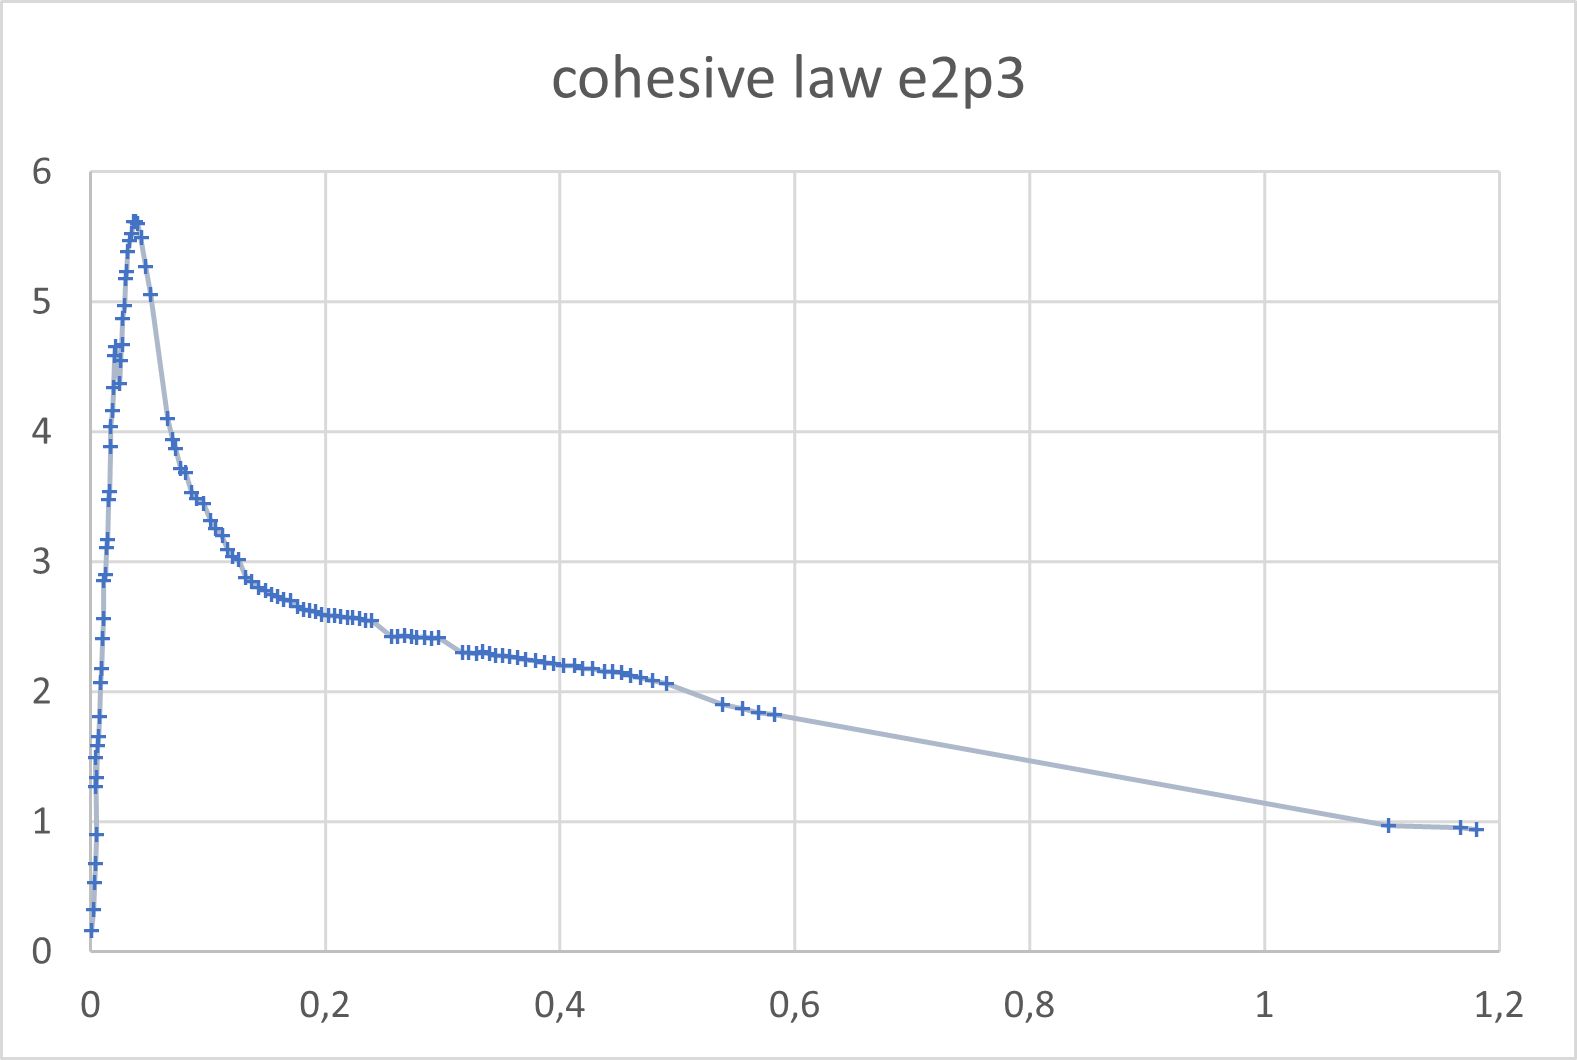
\includegraphics[scale=0.6]{Figures/e2p3_colaw}
	\decoRule
	\caption[Cohesive law from E2P3 specimen]{Cohesive law depending on the crack tip opening displacement and the energy release rate, for E2P3 specimen.}
	\label{fig:E2P3_colaw}
\end{subfigure}
\caption{Cohesive law from Okoume specimens at an average of 15\% moisture content}
\label{E2p_colaw}
\end{figure}
\newpage
%%%%%%%%%%%%%%%%%%%%%%%%%%%%%%%%%%%%%%%%%%%%%%%%%
%Section 3
%%%%%%%%%%%%%%%%%%%%%%%%%%%%%%%%%%%%%%%%%%%%%%%%%

\section{Results at 30\% Moisture Content}

\subsection{Crack length}

\begin{figure}[H]
\centering
\begin{subfigure}{0.48\linewidth}
	\centering
	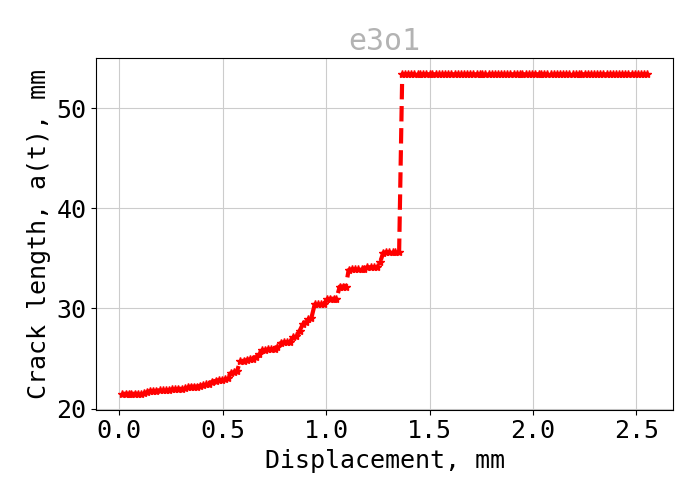
\includegraphics[scale=0.3]{Figures/e3o1_a}
	\decoRule
	\caption[Crack length E3O1]{Crack length depending on the press displacements, for E3O1 specimen.}
	\label{fig:E3O1_a}
\end{subfigure}
\hfill\\
\begin{subfigure}{0.48\linewidth}
	\centering
	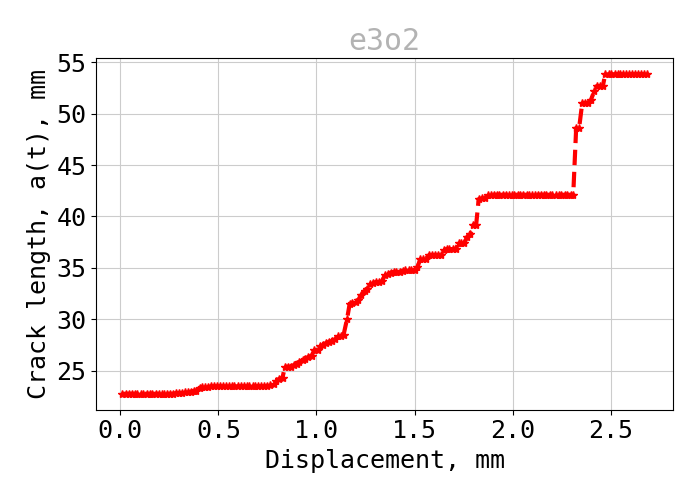
\includegraphics[scale=0.3]{Figures/e3o2_a}
	\decoRule
	\caption[Crack length E3O2]{Crack length depending on the press displacements, for E3O2 specimen.}
	\label{fig:E3O2_a}
\end{subfigure}
\hfill\\
\begin{subfigure}{0.48\linewidth}
	\centering
	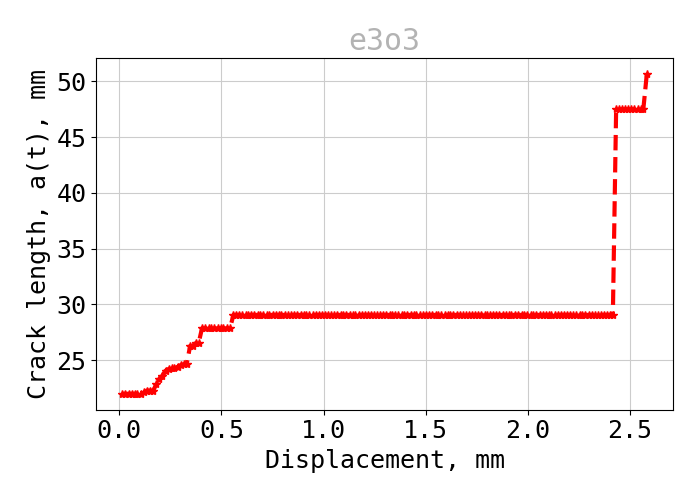
\includegraphics[scale=0.3]{Figures/e3o3_a}
	\decoRule
	\caption[Crack length E3O3]{Crack length depending on the press displacements, for E3O3 specimen.}
	\label{fig:E3O3_a}
\end{subfigure}
\caption{Crack length evolution on Okoume specimens at an average of 26\% moisture content}
\label{E3o_a}
\end{figure}
\newpage
\begin{figure}[H]
\centering
\begin{subfigure}{0.48\linewidth}
	\centering
	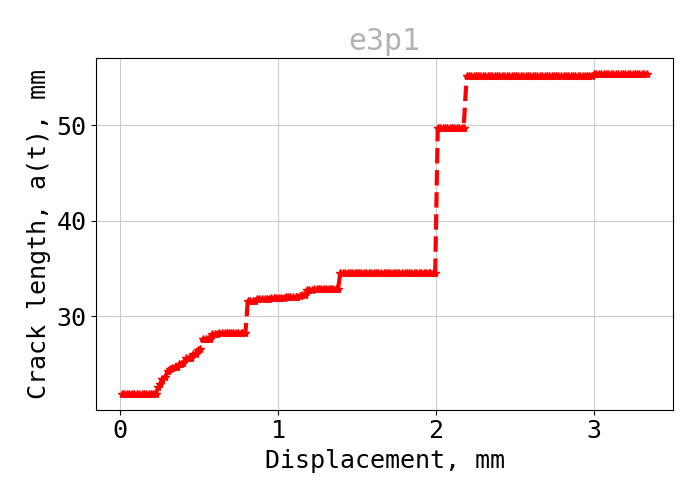
\includegraphics[scale=0.3]{Figures/e3p1_a}
	\decoRule
	\caption[Crack length E3P1]{Crack length depending on the press displacements, for E3P1 specimen.}
	\label{fig:E3P1_a}
\end{subfigure}
\hfill\\
\begin{subfigure}{0.48\linewidth}
	\centering
	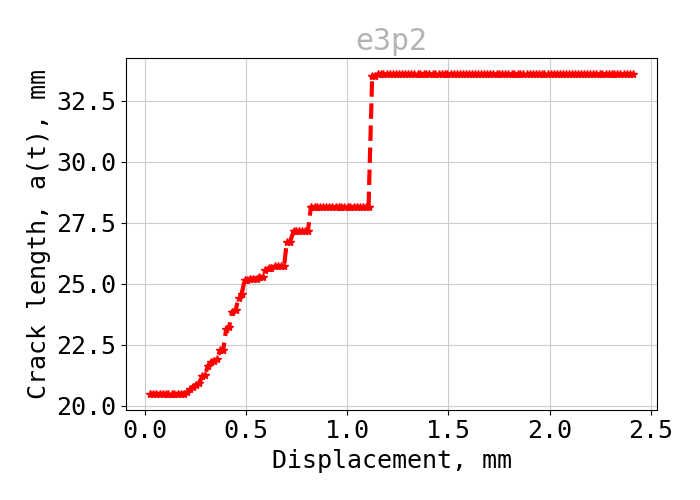
\includegraphics[scale=0.3]{Figures/e3p2_a}
	\decoRule
	\caption[Crack length E3P2]{Crack length depending on the press displacements, for E3P2 specimen.}
	\label{fig:E3P2_a}
\end{subfigure}
\hfill\\
\begin{subfigure}{0.48\linewidth}
	\centering
	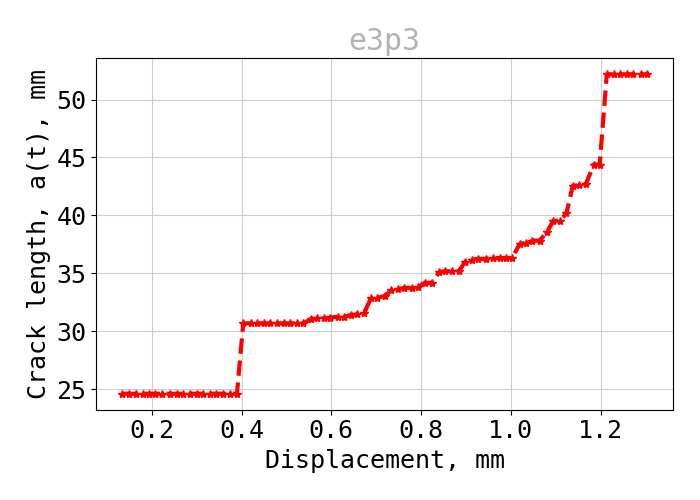
\includegraphics[scale=0.3]{Figures/e3p3_a}
	\decoRule
	\caption[Crack length E3P3]{Crack length depending on the press displacements, for E3P3 specimen.}
	\label{fig:E3P3_a}
\end{subfigure}
\caption{Crack length evolution on Padouck specimens at an average of 26\% moisture content}
\label{E3p_a}
\end{figure}
\newpage
\subsection{Energy release rate}

\begin{figure}[H]
\centering
\begin{subfigure}{0.48\linewidth}
	\centering
	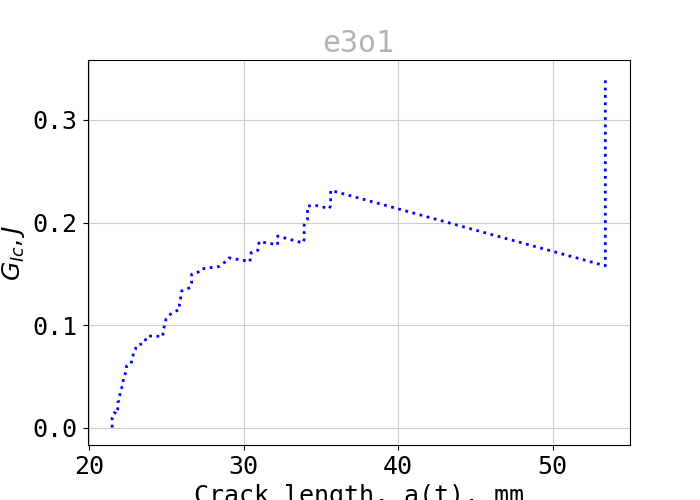
\includegraphics[scale=0.3]{Figures/e3o1_G}
	\decoRule
	\caption[Energy release rate E3O1]{Energy release rate depending on the crack length propagation, for E3O1 specimen.}
	\label{fig:E3O1_G}
\end{subfigure}
\hfill\\
\begin{subfigure}{0.48\linewidth}
	\centering
	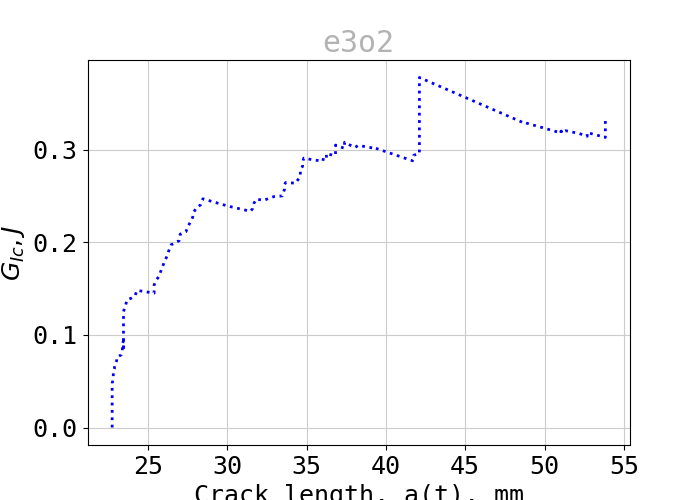
\includegraphics[scale=0.3]{Figures/e3o2_G}
	\decoRule
	\caption[Energy release rate E3O2]{Energy release rate depending on the crack length propagation, for E3O2 specimen.}
	\label{fig:E3O2_G}
\end{subfigure}
\hfill\\
\begin{subfigure}{0.48\linewidth}
	\centering
	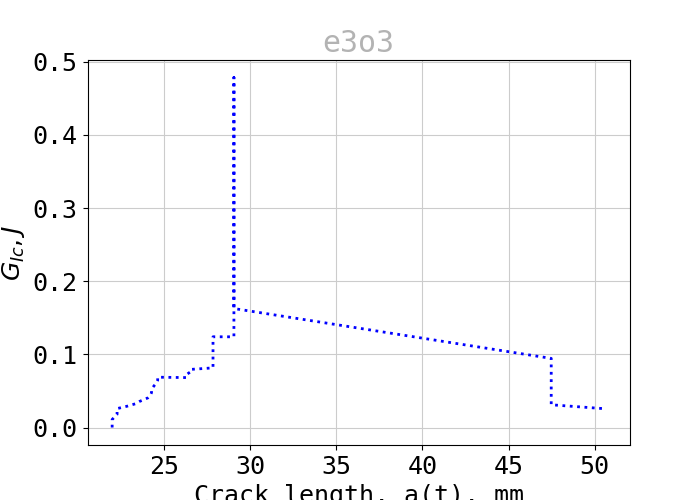
\includegraphics[scale=0.3]{Figures/e3o3_G}
	\decoRule
	\caption[Energy release rate E3O3]{Energy release rate depending on the crack length propagation, for E3O3 specimen.}
	\label{fig:E3O3_G}
\end{subfigure}
\caption{Energy release rate evolution on Okoume specimens at an average of 26\% moisture content}
\label{E3o_G}
\end{figure}
\newpage
\begin{figure}[H]
\centering
\begin{subfigure}{0.48\linewidth}
	\centering
	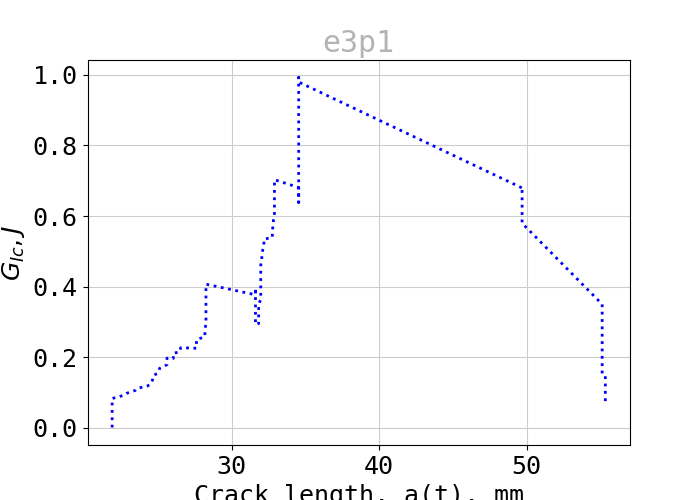
\includegraphics[scale=0.3]{Figures/e3p1_G}
	\decoRule
	\caption[Energy release rate E3P1]{Energy release rate depending on the crack length propagation, for E3P1 specimen.}
	\label{fig:E3P1_G}
\end{subfigure}
\hfill\\
\begin{subfigure}{0.48\linewidth}
	\centering
	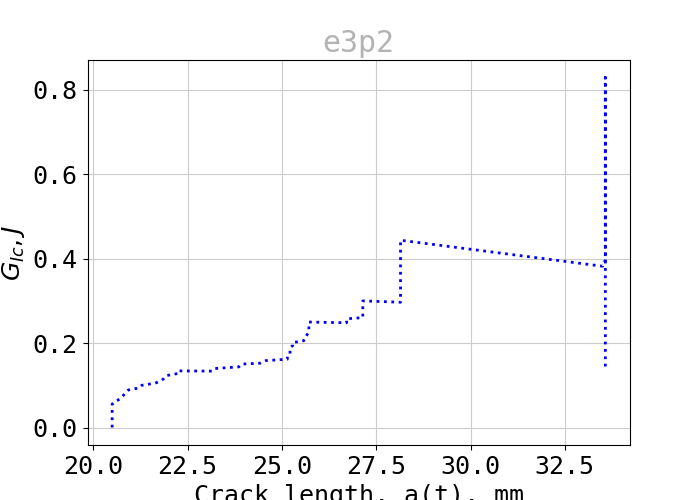
\includegraphics[scale=0.3]{Figures/e3p2_G}
	\decoRule
	\caption[Energy release rate E3P2]{Energy release rate depending on the crack length propagation, for E3P2 specimen.}
	\label{fig:E3P2_G}
\end{subfigure}
\hfill\\
\begin{subfigure}{0.48\linewidth}
	\centering
	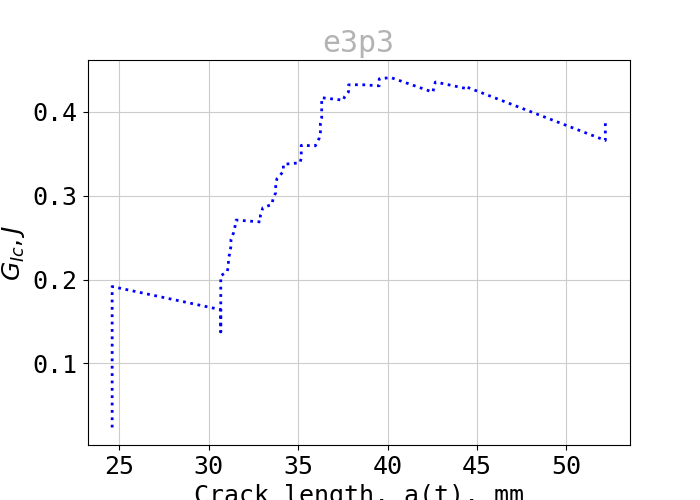
\includegraphics[scale=0.3]{Figures/e3p3_G}
	\decoRule
	\caption[Energy release rate E3P3]{Energy release rate depending on the crack length propagation, for E3P3 specimen.}
	\label{fig:E3P3_G}
\end{subfigure}
\caption{Energy release rate evolution on Padouck specimens at an average of 21\% moisture content}
\label{E3p_G}
\end{figure}
\newpage
\subsection{Cohesive law}

\begin{figure}[H]
\centering
\begin{subfigure}{0.48\linewidth}
	\centering
	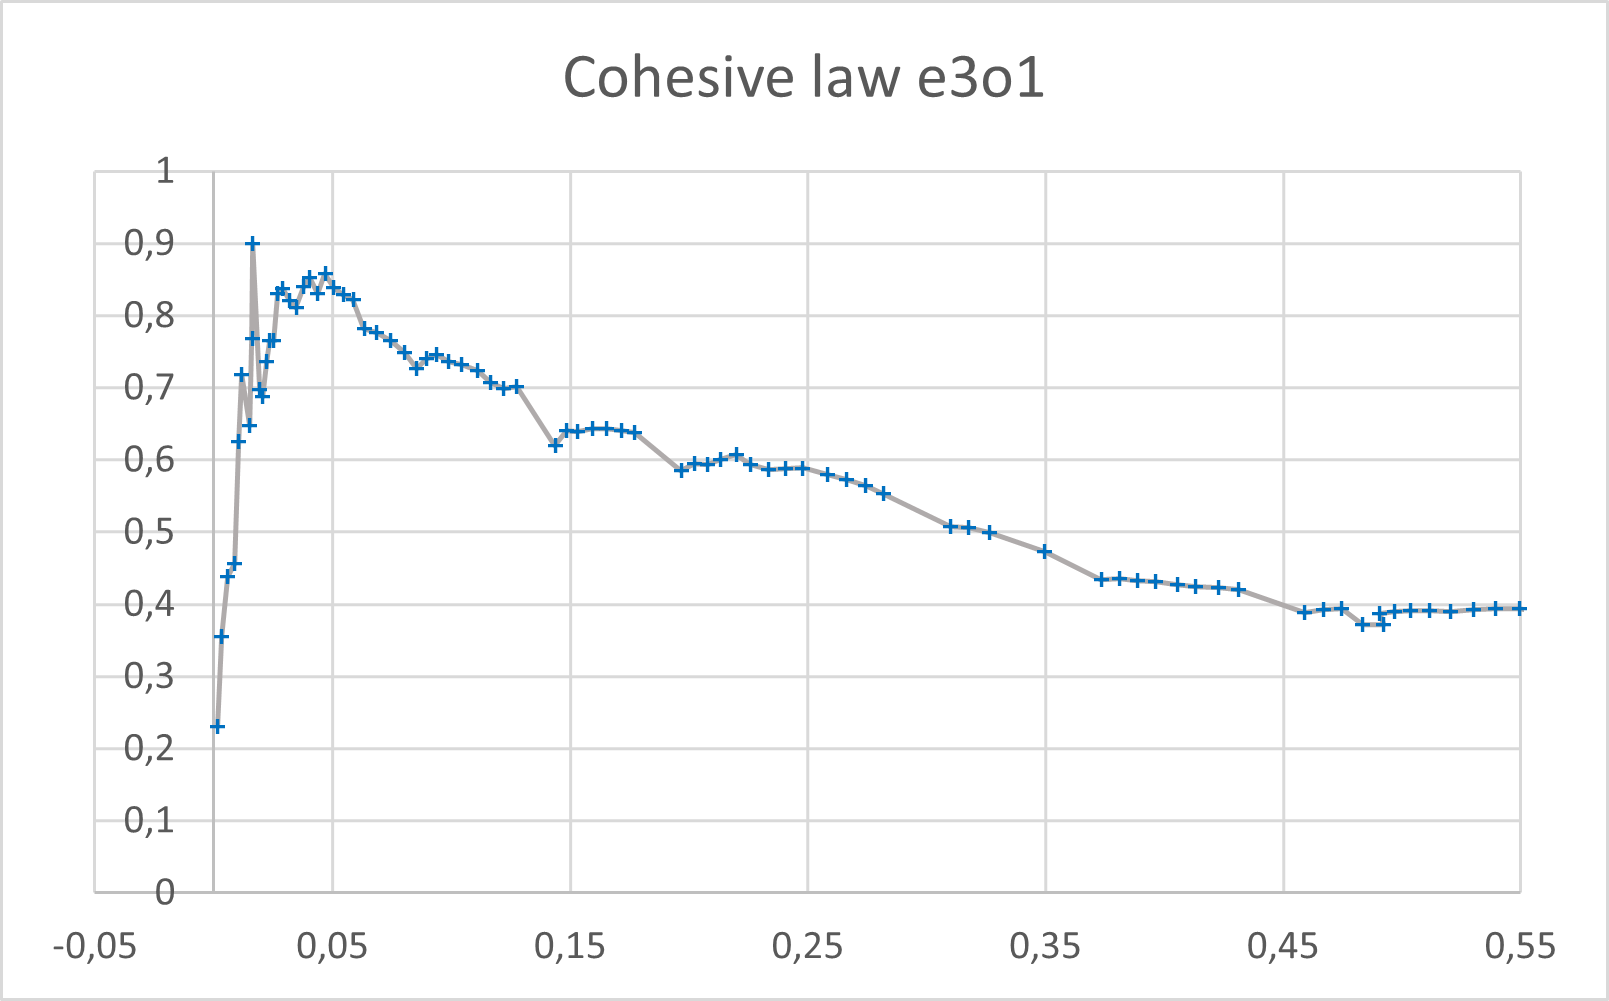
\includegraphics[scale=0.6]{Figures/e3o1_colaw}
	\decoRule
	\caption[Cohesive law from E3O1 specimen]{Cohesive law depending on the crack tip opening displacement and the energy release rate, for E3O1 specimen.}
	\label{fig:E3O1_colaw}
\end{subfigure}
\hfill\\
\begin{subfigure}{0.48\linewidth}
	\centering
	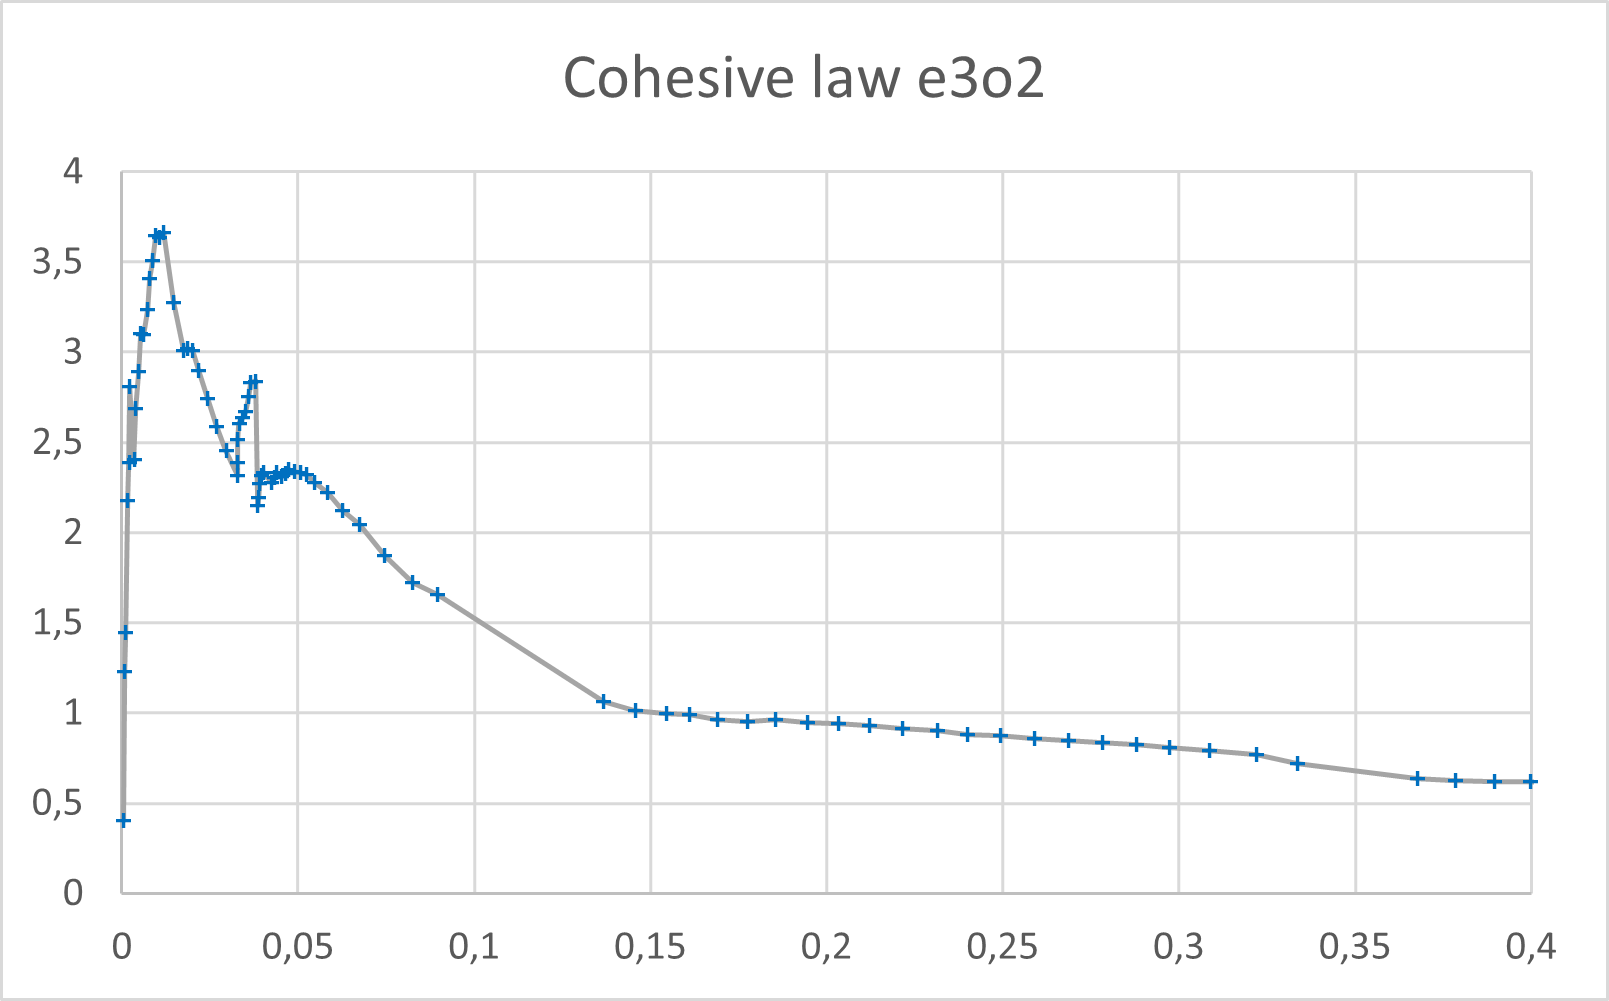
\includegraphics[scale=0.6]{Figures/e3o2_colaw}
	\decoRule
	\caption[Cohesive law from E3O2 specimen]{Cohesive law depending on the crack tip opening displacement and the energy release rate, for E3O2 specimen.}
	\label{fig:E3O2_colaw}
\end{subfigure}
\hfill\\
\begin{subfigure}{0.48\linewidth}
	\centering
	\includegraphics[scale=0.6]{Figures/e3o3_colaw}
	\decoRule
	\caption[Cohesive law from E3O3 specimen]{Cohesive law depending on the crack tip opening displacement and the energy release rate, for E3O3 specimen.}
	\label{fig:E3O3_colaw}
\end{subfigure}
\caption{Cohesive law from Okoume specimens at an average of 26\% moisture content}
\label{E3o_colaw}
\end{figure}
\newpage
\begin{figure}[H]
\centering
\begin{subfigure}{0.48\linewidth}
	\centering
	\includegraphics[scale=0.6]{Figures/e3p1_colaw}
	\decoRule
	\caption[Cohesive law from E3P1 specimen]{Cohesive law depending on the crack tip opening displacement and the energy release rate, for E3P1 specimen.}
	\label{fig:E3P1_colaw}
\end{subfigure}
\hfill\\
\begin{subfigure}{0.48\linewidth}
	\centering
	\includegraphics[scale=0.6]{Figures/e3p2_colaw}
	\decoRule
	\caption[Cohesive law from E3P2 specimen]{Cohesive law depending on the crack tip opening displacement and the energy release rate, for E3P2 specimen.}
	\label{fig:E3P2_colaw}
\end{subfigure}
\hfill\\
\begin{subfigure}{0.48\linewidth}
	\centering
	\includegraphics[scale=0.6]{Figures/e3p3_colaw}
	\decoRule
	\caption[Cohesive law from E3P3 specimen]{Cohesive law depending on the crack tip opening displacement and the energy release rate, for E3P3 specimen.}
	\label{fig:E3P3_colaw}
\end{subfigure}
\caption{Cohesive law from Okoume specimens at an average of 21\% moisture content}
\label{E3p_colaw}
\end{figure}


%\textbf{\textit{\underline{TO CHANGE DEPENDING ON MC AFTER LAST DRY}}} 
%Replace nu by $\nu_{RT}$
%ER by $E_{R}$
%GRT by $G_{RT}$
%
%
%\begin{table}[]
%	\centering
%	\begin{tabular}{lcccc}
%		\cline{2-5}
%		\multicolumn{1}{l|}{} & \multicolumn{1}{l|}{\cellcolor[HTML]{FCD5B4}Okoumé} & \multicolumn{1}{l|}{\cellcolor[HTML]{E26B0A}Padouck} & \multicolumn{1}{l|}{\cellcolor[HTML]{CC9900}Iroko} & \multicolumn{1}{l|}{\cellcolor[HTML]{D9D9D9}Silver Fir} \\ \hline
%		\multicolumn{1}{|l|}{F=hardwood / R=softwood} & \multicolumn{1}{c|}{F} & \multicolumn{1}{c|}{F} & \multicolumn{1}{c|}{F} & \multicolumn{1}{c|}{R} \\ \hline
%		\multicolumn{1}{|l|}{Air-Dry   density} & \multicolumn{1}{c|}{0,44} & \multicolumn{1}{c|}{0,79} & \multicolumn{1}{c|}{0,64} & \multicolumn{1}{c|}{0,52} \\ \hline
%		\multicolumn{1}{|l|}{Humidity} & \multicolumn{1}{c|}{12} & \multicolumn{1}{c|}{12} & \multicolumn{1}{c|}{12} & \multicolumn{1}{c|}{12} \\ \hline
%		\multicolumn{1}{|l|}{Temperature   °C} & \multicolumn{1}{c|}{20} & \multicolumn{1}{c|}{20} & \multicolumn{1}{c|}{20} & \multicolumn{1}{c|}{20} \\ \hline
%		& \multicolumn{1}{l}{} & \multicolumn{1}{l}{} & \multicolumn{1}{l}{} & \multicolumn{1}{l}{} \\ \hline
%		\multicolumn{1}{|l|}{ER} & \multicolumn{1}{c|}{1089,883} & \multicolumn{1}{c|}{2332,418} & \multicolumn{1}{c|}{1773,884} & \multicolumn{1}{c|}{1165,900} \\ \hline
%		\multicolumn{1}{|l|}{ET} & \multicolumn{1}{c|}{522,367} & \multicolumn{1}{c|}{1446,236} & \multicolumn{1}{c|}{1002,585} & \multicolumn{1}{c|}{769,700} \\ \hline
%		\multicolumn{1}{|l|}{EL} & \multicolumn{1}{c|}{9634,252} & \multicolumn{1}{c|}{17604,255} & \multicolumn{1}{c|}{14171,868} & \multicolumn{1}{c|}{16019,000} \\ \hline
%		\multicolumn{1}{|l|}{GTL} & \multicolumn{1}{c|}{593,880} & \multicolumn{1}{c|}{1241,534} & \multicolumn{1}{c|}{952,215} & \multicolumn{1}{c|}{814,230} \\ \hline
%		\multicolumn{1}{|l|}{GRL} & \multicolumn{1}{c|}{807,580} & \multicolumn{1}{c|}{1573,781} & \multicolumn{1}{c|}{1237,925} & \multicolumn{1}{c|}{1006,600} \\ \hline
%		\multicolumn{1}{|l|}{GRT} & \multicolumn{1}{c|}{185,618} & \multicolumn{1}{c|}{513,905} & \multicolumn{1}{c|}{356,258} & \multicolumn{1}{c|}{99,560} \\ \hline
%		\multicolumn{1}{|l|}{QTL} & \multicolumn{1}{c|}{-20391,184} & \multicolumn{1}{c|}{-38591,580} & \multicolumn{1}{c|}{-30677,164} & \multicolumn{1}{c|}{-37870,000} \\ \hline
%		\multicolumn{1}{|l|}{QRL} & \multicolumn{1}{c|}{-26121,086} & \multicolumn{1}{c|}{-44571,010} & \multicolumn{1}{c|}{-36775,726} & \multicolumn{1}{c|}{-35019,000} \\ \hline
%		\multicolumn{1}{|l|}{QRT} & \multicolumn{1}{c|}{-1545,949} & \multicolumn{1}{c|}{-3528,427} & \multicolumn{1}{c|}{-2622,049} & \multicolumn{1}{c|}{-2419,600} \\ \hline
%		\multicolumn{1}{|l|}{$\nu_{RT}$} & \multicolumn{1}{c|}{0,705} & \multicolumn{1}{c|}{0,661} & \multicolumn{1}{c|}{0,677} & \multicolumn{1}{c|}{0,482} \\ \hline
%		\multicolumn{1}{|l|}{$\nu_{TR}$} & \multicolumn{1}{c|}{0,338} & \multicolumn{1}{c|}{0,410} & \multicolumn{1}{c|}{0,382} & \multicolumn{1}{c|}{0,318} \\ \hline
%		\multicolumn{1}{|l|}{nuRL} & \multicolumn{1}{c|}{0,042} & \multicolumn{1}{c|}{0,052} & \multicolumn{1}{c|}{0,048} & \multicolumn{1}{c|}{0,033} \\ \hline
%		\multicolumn{1}{|l|}{nuLR} & \multicolumn{1}{c|}{0,369} & \multicolumn{1}{c|}{0,395} & \multicolumn{1}{c|}{0,385} & \multicolumn{1}{c|}{0,457} \\ \hline
%		\multicolumn{1}{|l|}{nuTL} & \multicolumn{1}{c|}{0,026} & \multicolumn{1}{c|}{0,037} & \multicolumn{1}{c|}{0,033} & \multicolumn{1}{c|}{0,020} \\ \hline
%		\multicolumn{1}{|l|}{nuLT} & \multicolumn{1}{c|}{0,472} & \multicolumn{1}{c|}{0,456} & \multicolumn{1}{c|}{0,462} & \multicolumn{1}{c|}{0,423} \\ \hline
%	\end{tabular}
%	\caption{Guitard values obtained by adding volumic weight, ambient temperature and ambient relative humidty
%	}
%	\label{tab:Tab1}
%\end{table}
%Thanks to this values obtained with Guitard model, it is possible to have the D matrix needed for Abaqus processing.
%\section{D matrix values} 
% Please add the following required packages to your document preamble:
% \usepackage[table,xcdraw]{xcolor}
% If you use beamer only pass "xcolor=table" option, i.e. \documentclass[xcolor=table]{beamer}
%\begin{table}[]
%	\centering
%	\begin{tabular}{l|c|c|c|}
%		\cline{2-4}
%		& \cellcolor[HTML]{F8CBAD}Okoume & \cellcolor[HTML]{BF8F00}Iroko & \cellcolor[HTML]{C65911}Padock \\ \hline
%		\multicolumn{1}{|l|}{D1111} & 10178,7919 & 14036,2632 & 19105,7691 \\ \hline
%		\multicolumn{1}{|l|}{D2222} & 1493,14142 & 1933,3864 & 3412,12799 \\ \hline
%		\multicolumn{1}{|l|}{D3333} & 551,518515 & 820,343041 & 1569,35595 \\ \hline
%		\multicolumn{1}{|l|}{D1122} & 798,553338 & 1265,04277 & 2020,01424 \\ \hline
%		\multicolumn{1}{|l|}{D1133} & 529,927394 & 869,687844 & 1543,56016 \\ \hline
%		\multicolumn{1}{|l|}{D2233} & 524,542701 & 774,648324 & 1474,17476 \\ \hline
%		\multicolumn{1}{|l|}{D1212} & 808 & 1040 & 1574 \\ \hline
%		\multicolumn{1}{|l|}{D1313} & 594 & 800 & 1242 \\ \hline
%		\multicolumn{1}{|l|}{D2323} & 186 & 279 & 514 \\ \hline
%	\end{tabular}
%	\caption{D matrix linked to Guitard values}
%	\label{tab:Tab10}
%\end{table}

